\chapter{Non-Uniform Cryogenic Targets}
  As discussed in Section 5.4.2, the cryogenic targets (cryo-target) used in the E08-014, $\mathrm{^{2}H}$, $\mathrm{^{3}He}$ and $\mathrm{^{4}He}$, presented strange distributions in $z_{react}$. These distributions indicate that their densities were not uniform but instead, vary along the 20~cm cells. As proved by a Monte Carlo simulation of the cryogenic target system~\cite{silviu_target},  such non-uniform density profiles were caused by the poor design of the target cells and the direction of the cryogenic flow, as shown in Fig.~\ref{silviu_plots}.
\begin{figure}[!ht]
  \begin{center}
    \subfloat[$\mathrm{^{2}H}$]{
      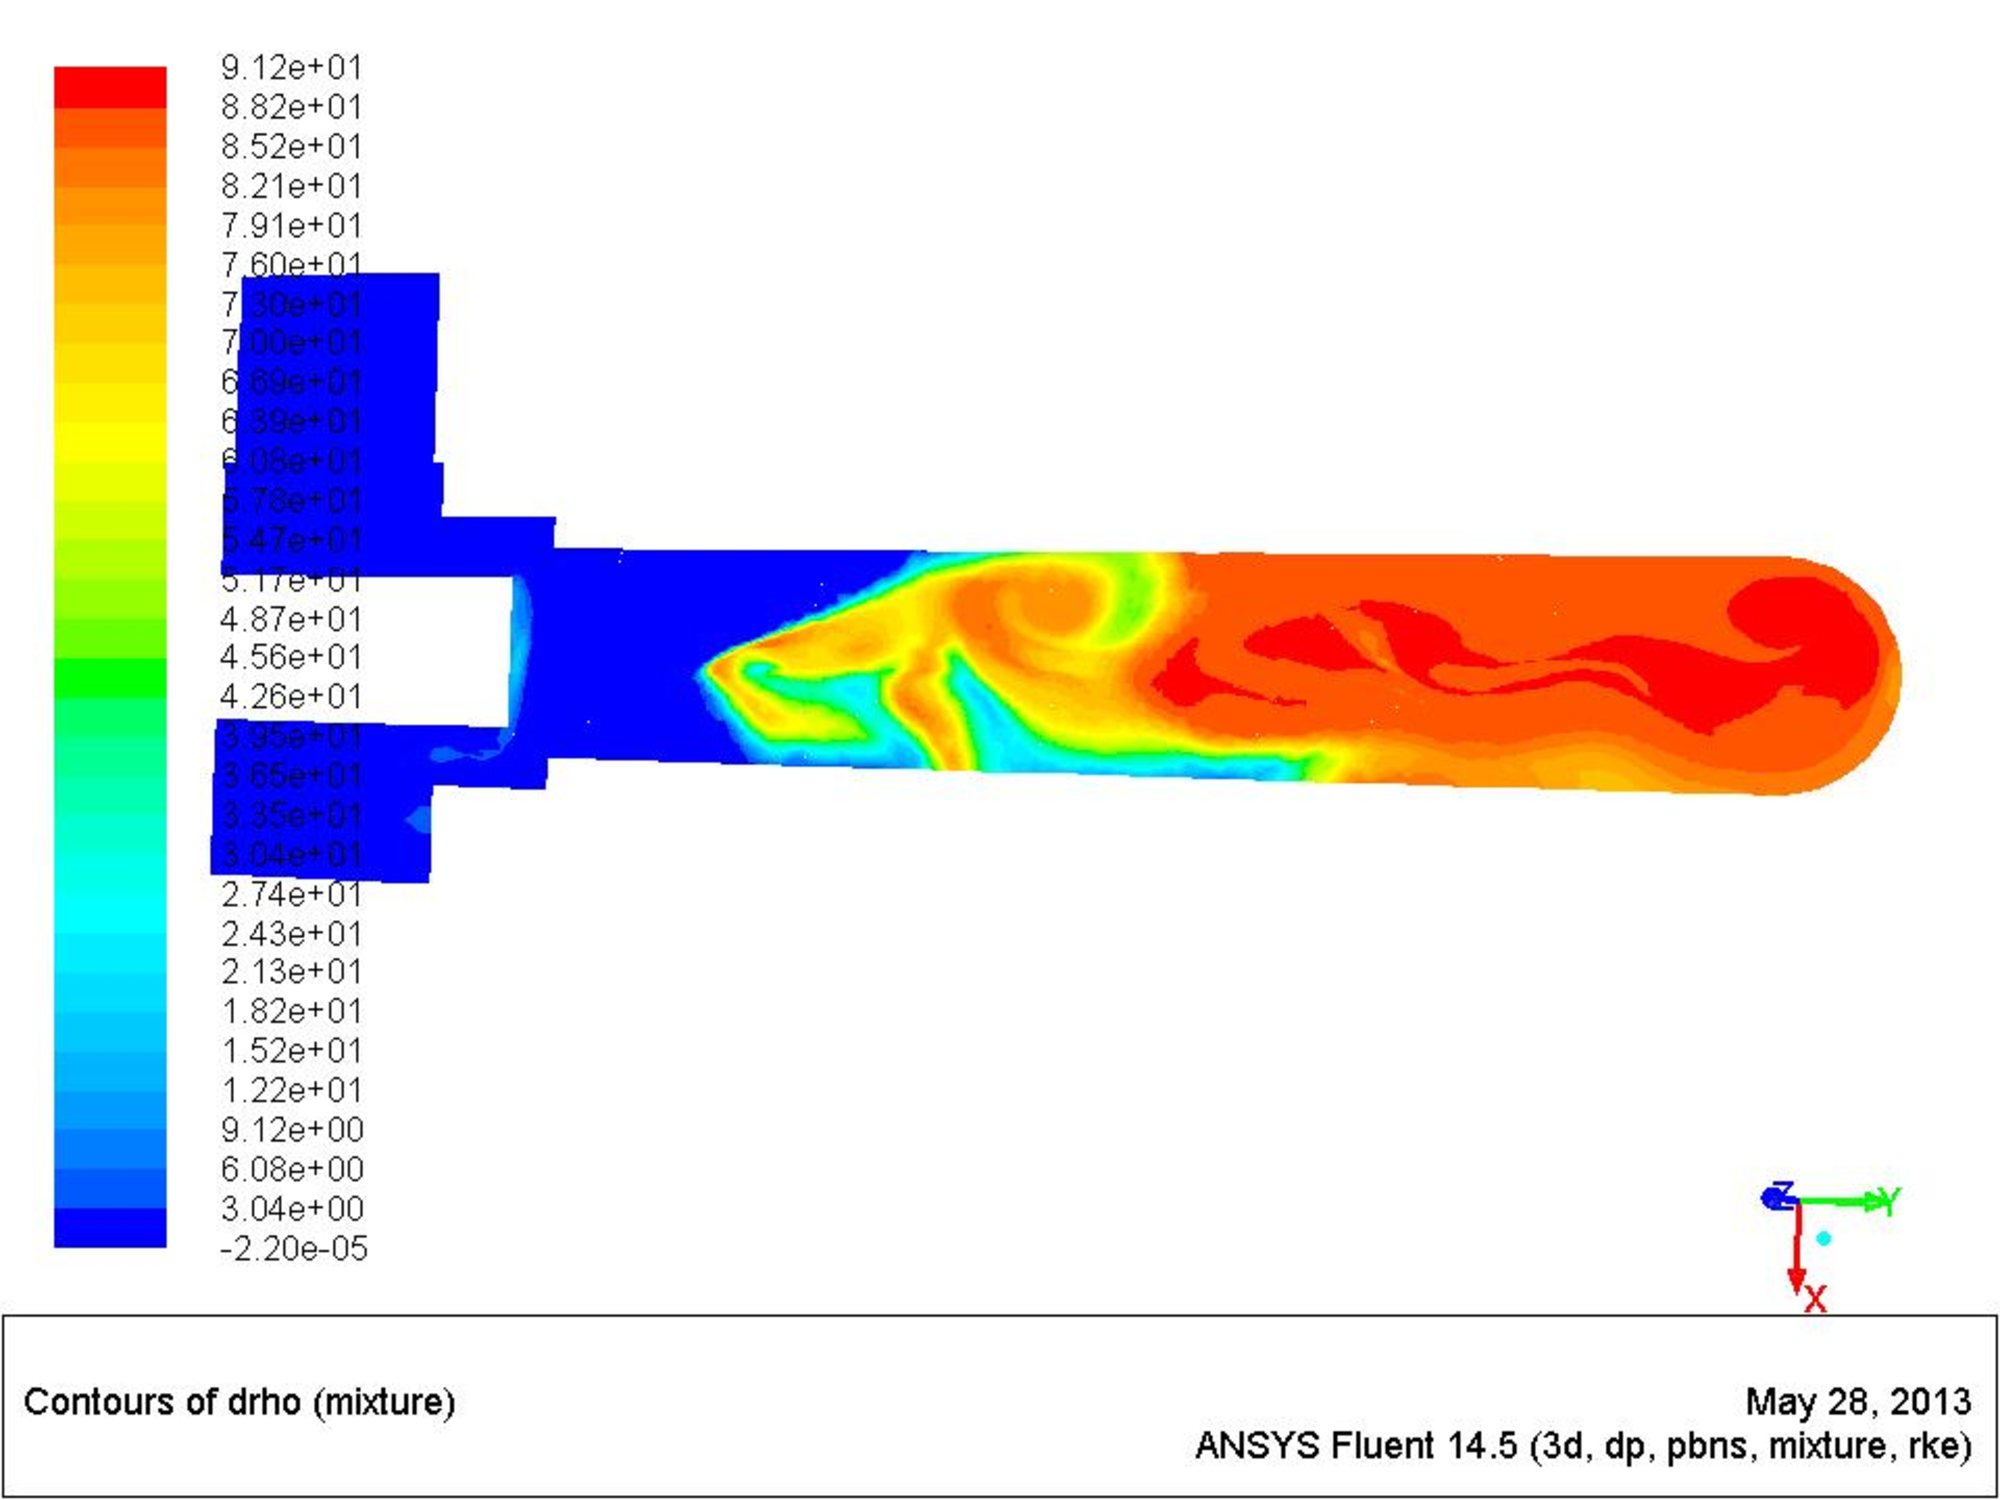
\includegraphics[type=pdf,ext=.pdf,read=.pdf,width=0.45\textwidth]{./figures/target/LD2_density} 
    }
    \hfill
     \subfloat[$\mathrm{^{4}He}$]{
      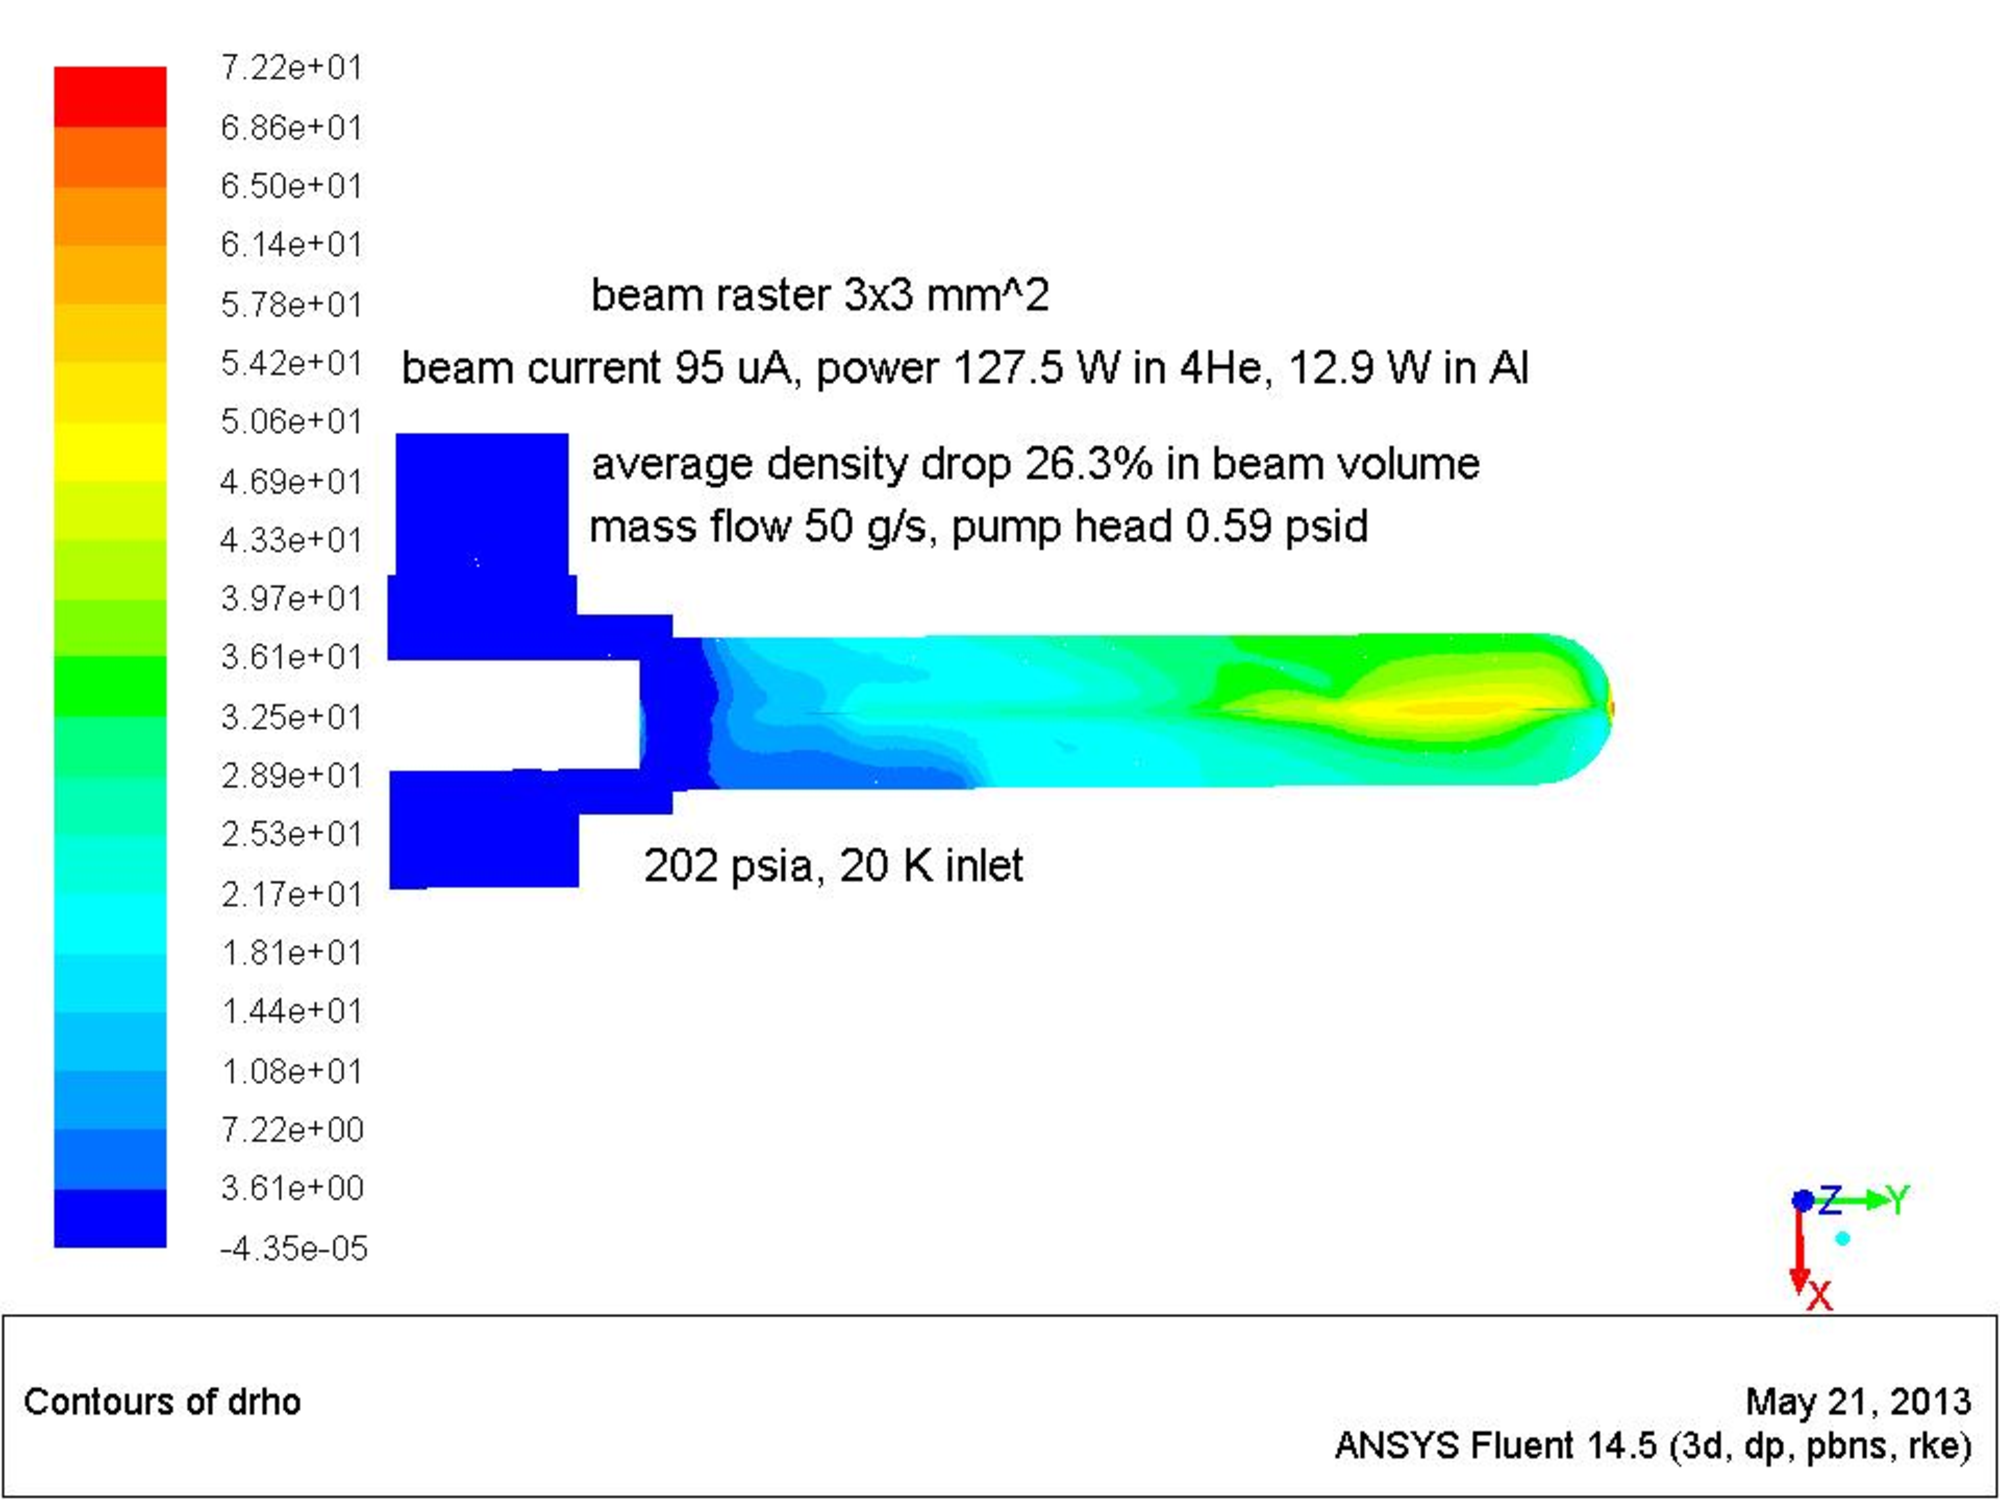
\includegraphics[type=pdf,ext=.pdf,read=.pdf,width=0.45\textwidth]{./figures/target/He4_density} 
    }
    \caption[Cryo-target density profiles from simulation]{\footnotesize{Cryo-target density profiles from simulation. The color contour denotes the value of the target density. The left plot is for $\mathrm{^{2}H}$ and the right plot is for $\mathrm{^{4}He}$. The density profile of $\mathrm{^{3}He}$ is not shown here. Both plots present the fluctuations of the target density along the cell.}}
    \label{silviu_plots}
  \end{center}
\end{figure}
 
  The absolute target density is required in order to extract the cross sections. The initial target density with the beam off can be determined before the experiment. When the beam is on, however, the density varies with the beam current because of the boiling effect. Such an effect is negligible for solid targets but it could be significant for cryo-targets. For a non-uniform cryo-target, the boiling effect differs along the target cell, and in addition, the radiation correction becomes more complicated since the radiation effect largely depends on the location and direction of the electron-scattering process. In this chapter, a detailed study of the boiling effect is given, followed by a discussion of extracting the cryo-target density distributions. A procedure to evaluate the radiation correction factors for non-uniform cryo-targets will be introduced in the end.

\section{Boiling Study}
 \begin{figure}[!ht]
  \begin{center}
    \subfloat[$\mathrm{^{12}C}$ on HRS-L]{
      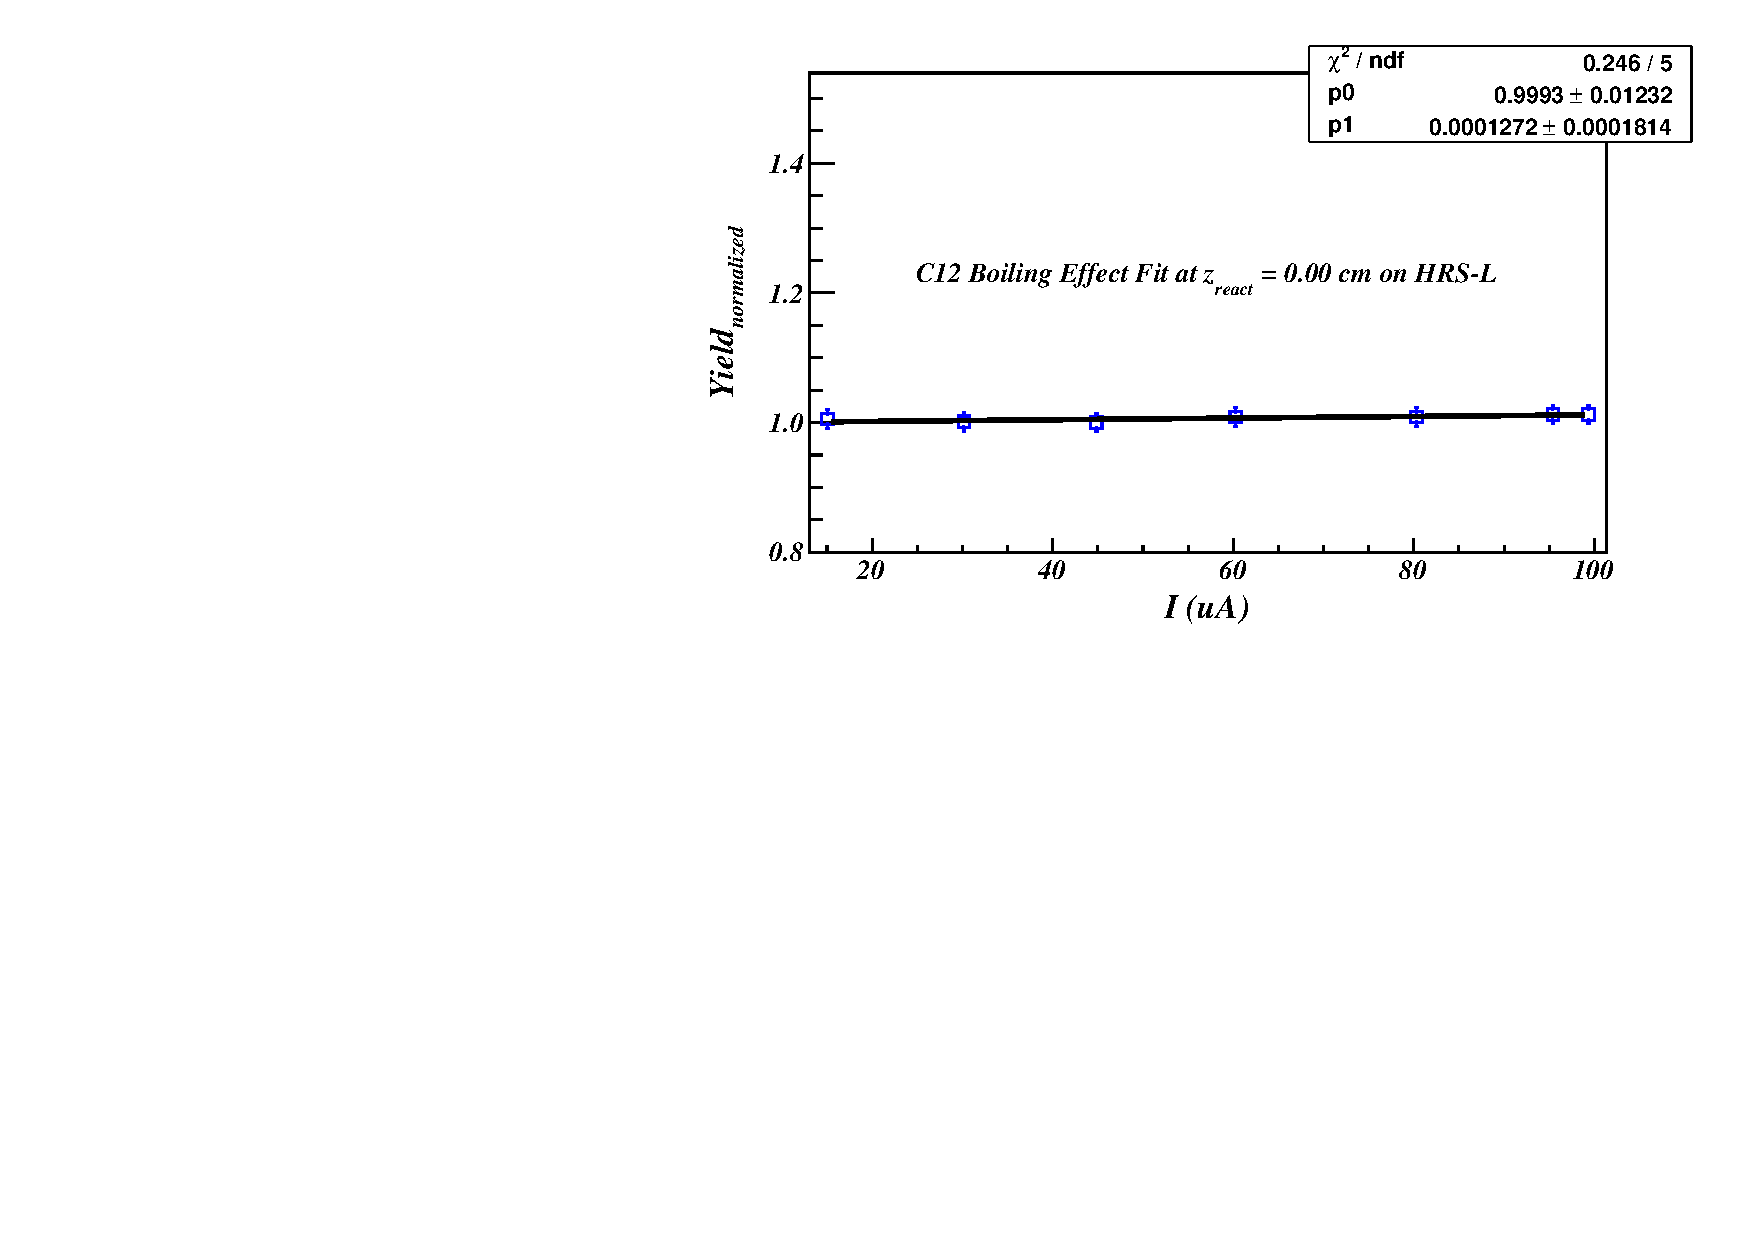
\includegraphics[type=pdf,ext=.pdf,read=.pdf,width=0.45\textwidth]{./figures/cryo/C12_Yield_L_All_0} 
    }
    \hfill
    \subfloat[$\mathrm{^{12}C}$ on HRS-R]{
      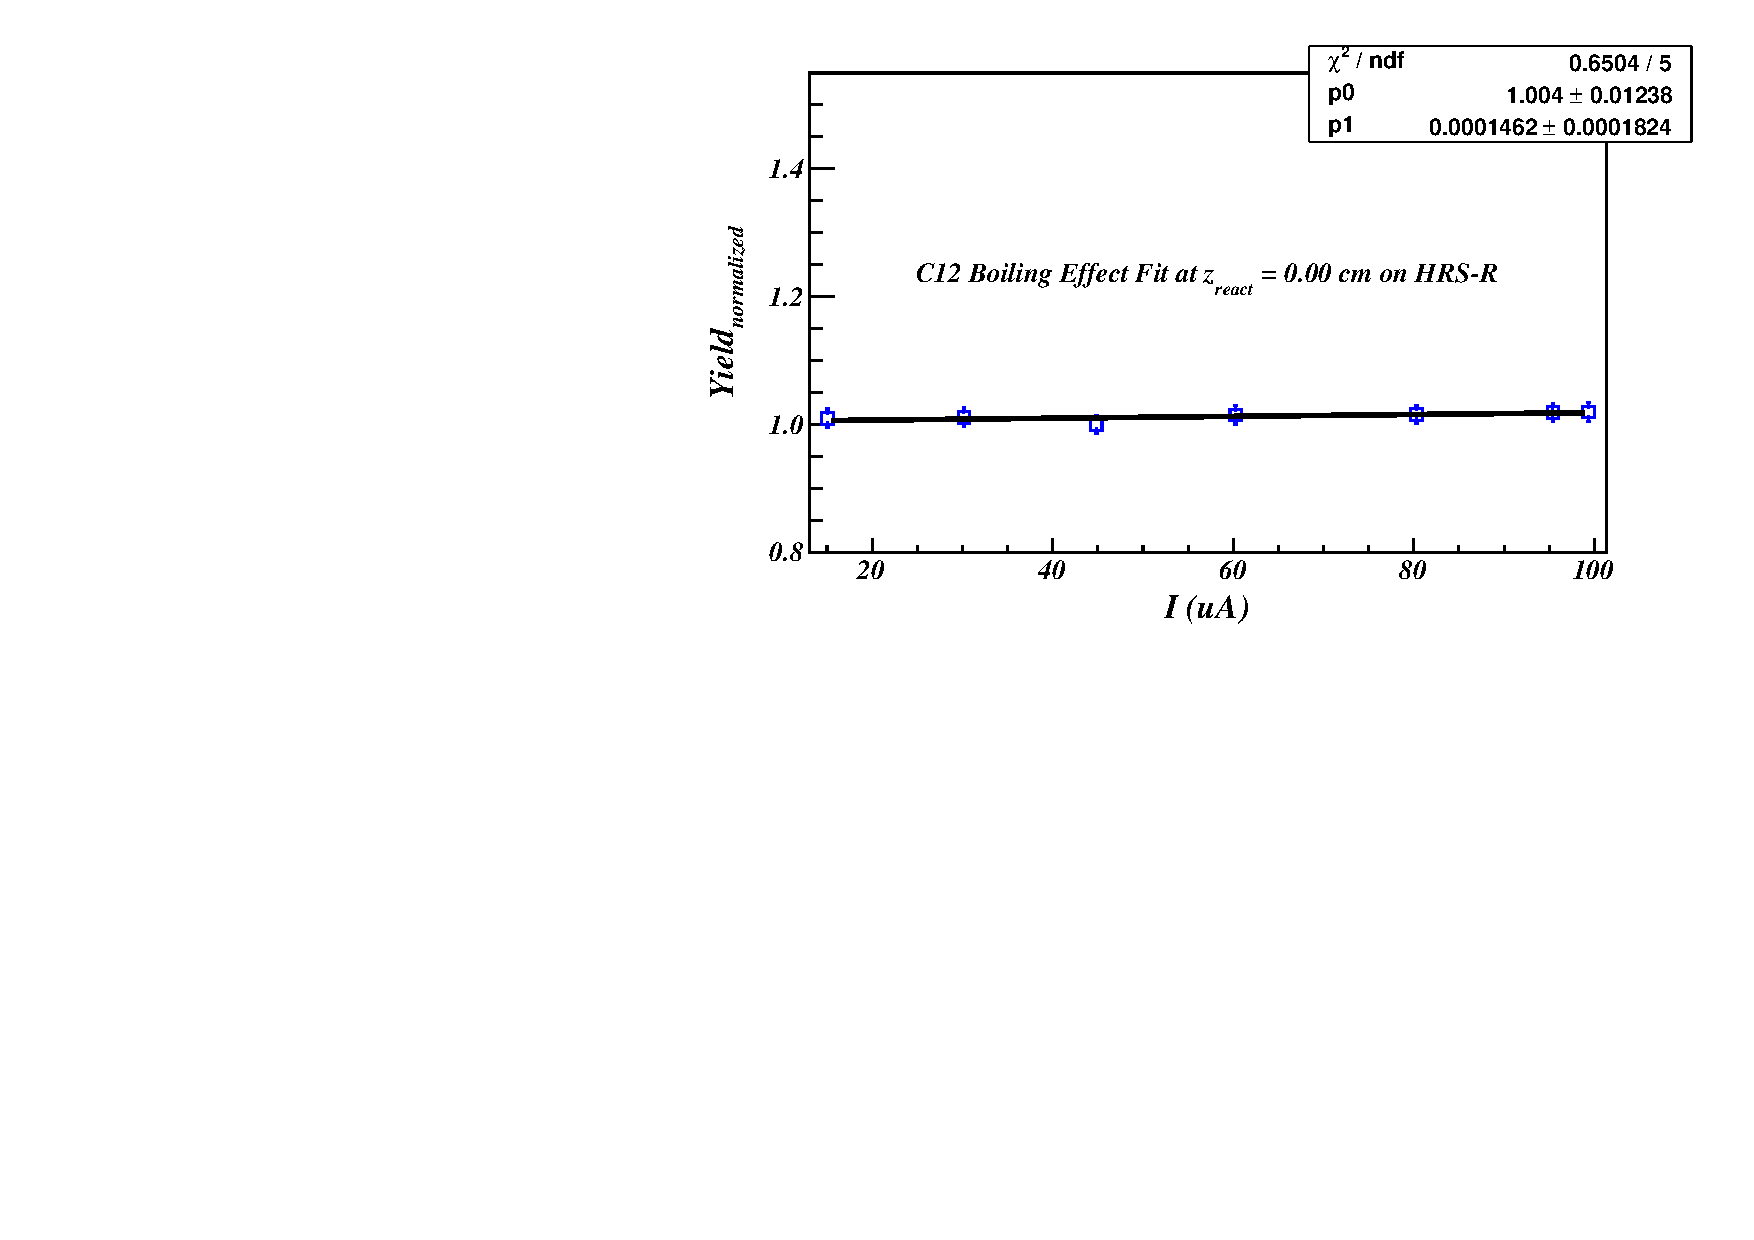
\includegraphics[type=pdf,ext=.pdf,read=.pdf,width=0.45\textwidth]{./figures/cryo/C12_Yield_R_All_0} 
    }
    \caption[$\mathrm{^{12}C}$ boiling effect fitting]{\footnotesize{$\mathrm{^{12}C}$ boiling effect fitting. Since $\mathrm{^{12}C}$ should have very small boiling effect, this study is used to check any rate-dependence effect at different current settings. The yield values have been normalized by a common factor.}}
    \label{c12_boil_fit}
  \end{center}
\end{figure}
  During the E08-014, several boiling study runs were taken with different beam current on these cryo-targets, as well as on the $\mathrm{^{12}C}$ target which was used to check any rate-dependence effects.
  
  The experimental yield depends on the target density, the beam charge and the cross section of electron-nucleus scattering. While the average cross section shouldn't change for one kinematic setting, the yield normalized by the beam charge should be directly proportional to the target density:
\begin{equation}
  Y(I) = Y(0) + m\cdot I,
  \label{eq_yield_boiling}
\end{equation}  
where $Y(I)$, the yield for one run with the beam current $I$, is equal to the total number of experimental events after all necessary cuts divided by the the total accumulated charge. $Y(0)$ is the yield extrapolated to zero beam current and $m$ is the slop of $Y(I)$ on $I$. By fitting Eq.~\eqref{eq_yield_boiling} with the data of the boiling study runs, one can obtain the variation of the target density at different current, given as:
\begin{equation}
  \rho(I) = \rho(0) \cdot (1.0 + BF \cdot I /100),
  \label{eq_yield_rho}
\end{equation}
where $BF=Y(0)/m$ is the boiling factor of the target.

\begin{figure}[!h]
  \begin{center}
    \subfloat[$\mathrm{^{2}H}$ on HRS-L]{
      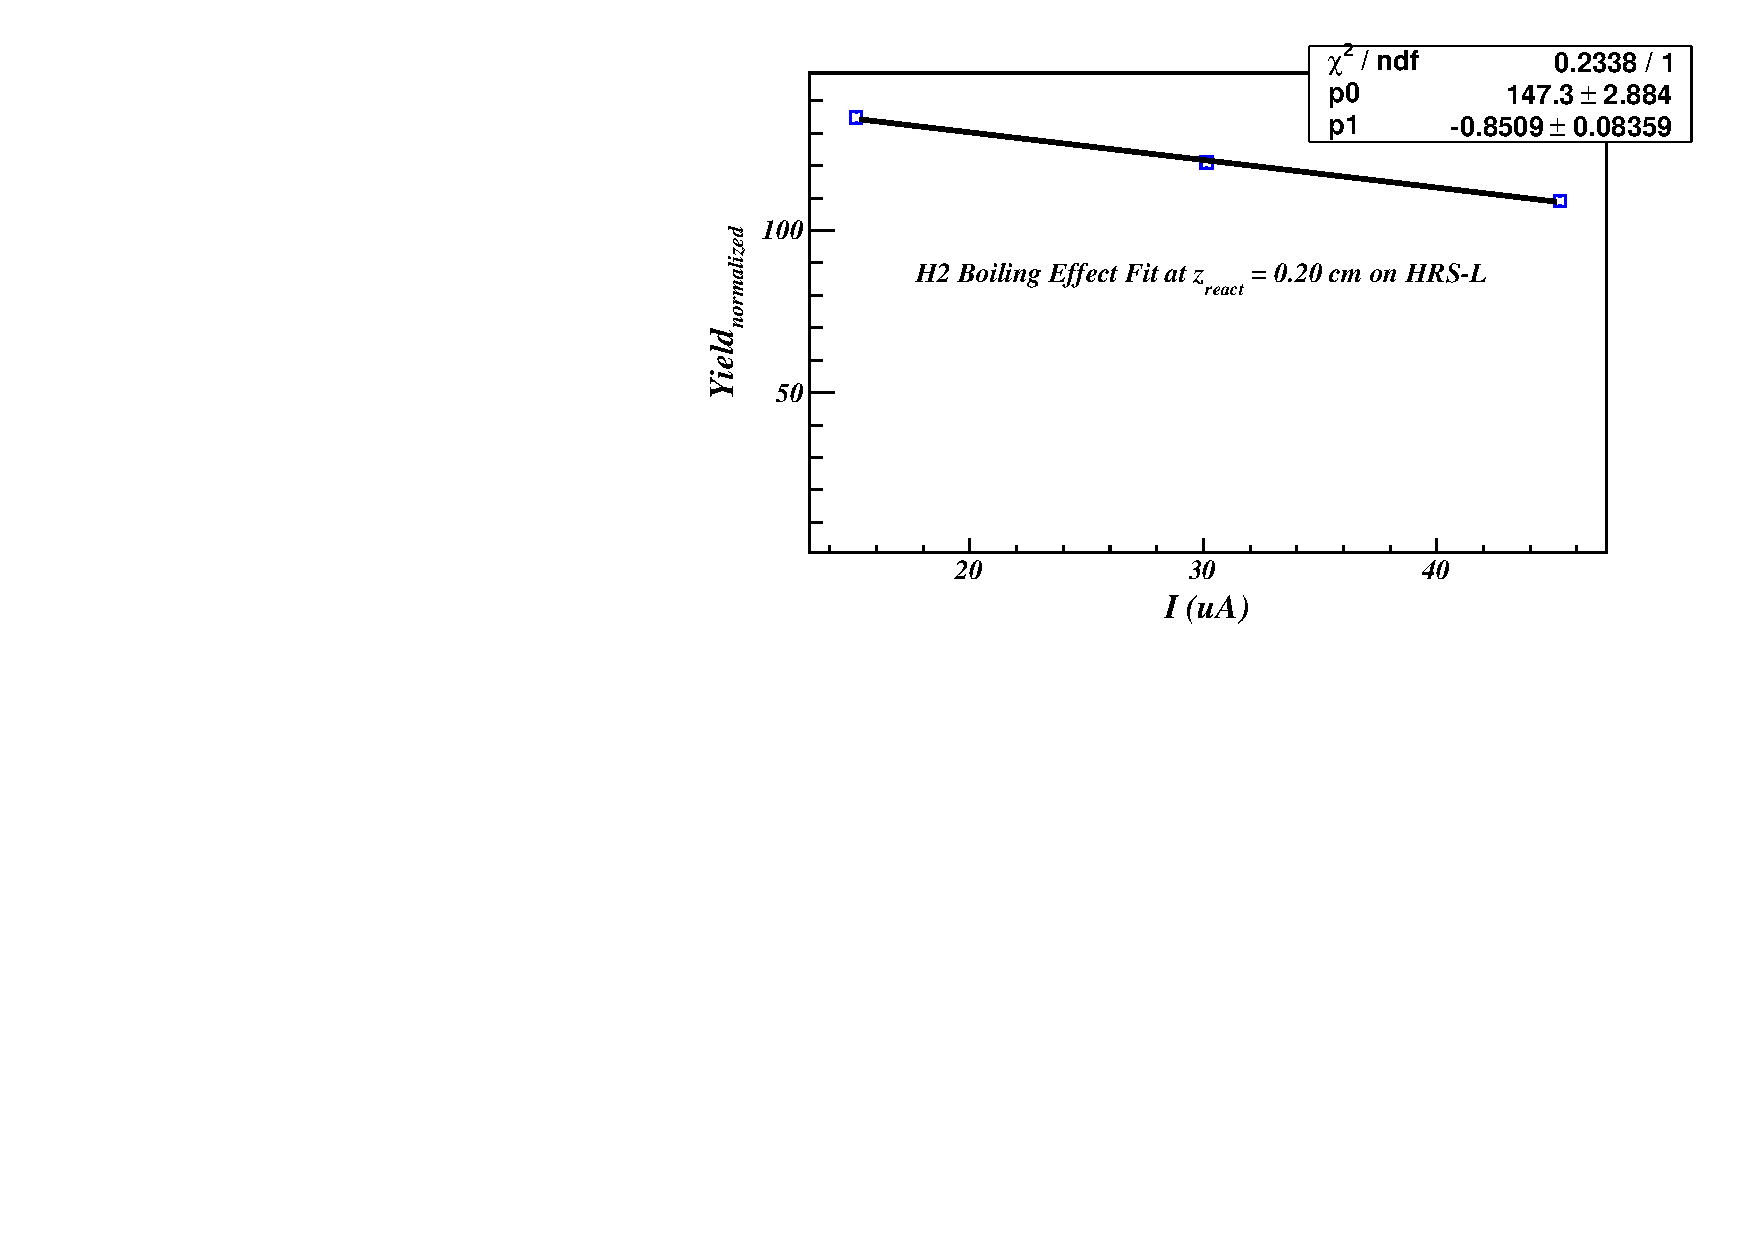
\includegraphics[type=pdf,ext=.pdf,read=.pdf,width=0.45\textwidth]{./figures/cryo/H2_Yield_L_All_0} 
    }
    \hfill
    \subfloat[$\mathrm{^{2}H}$ on HRS-R]{
      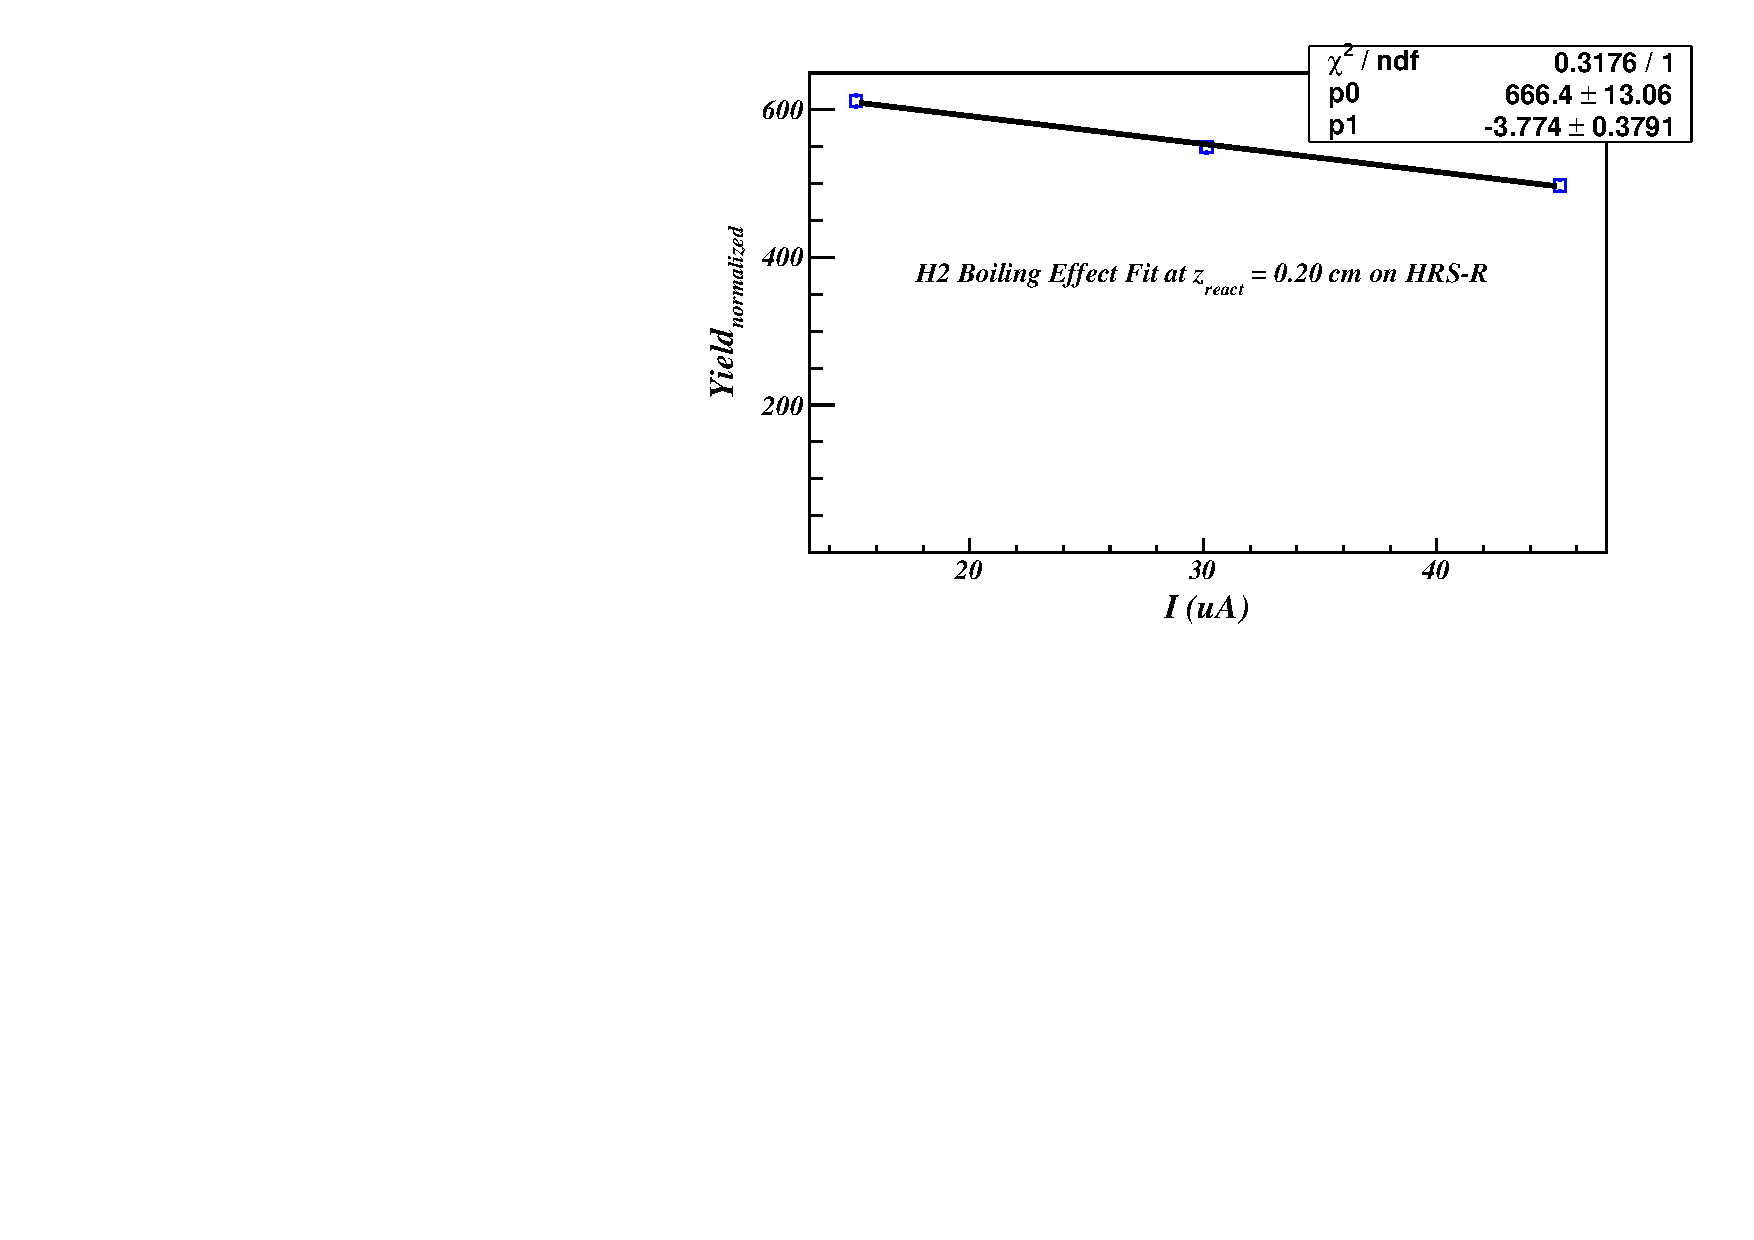
\includegraphics[type=pdf,ext=.pdf,read=.pdf,width=0.45\textwidth]{./figures/cryo/H2_Yield_R_All_0} 
    }
\\
    \subfloat[$\mathrm{^{3}He}$ on HRS-L]{
      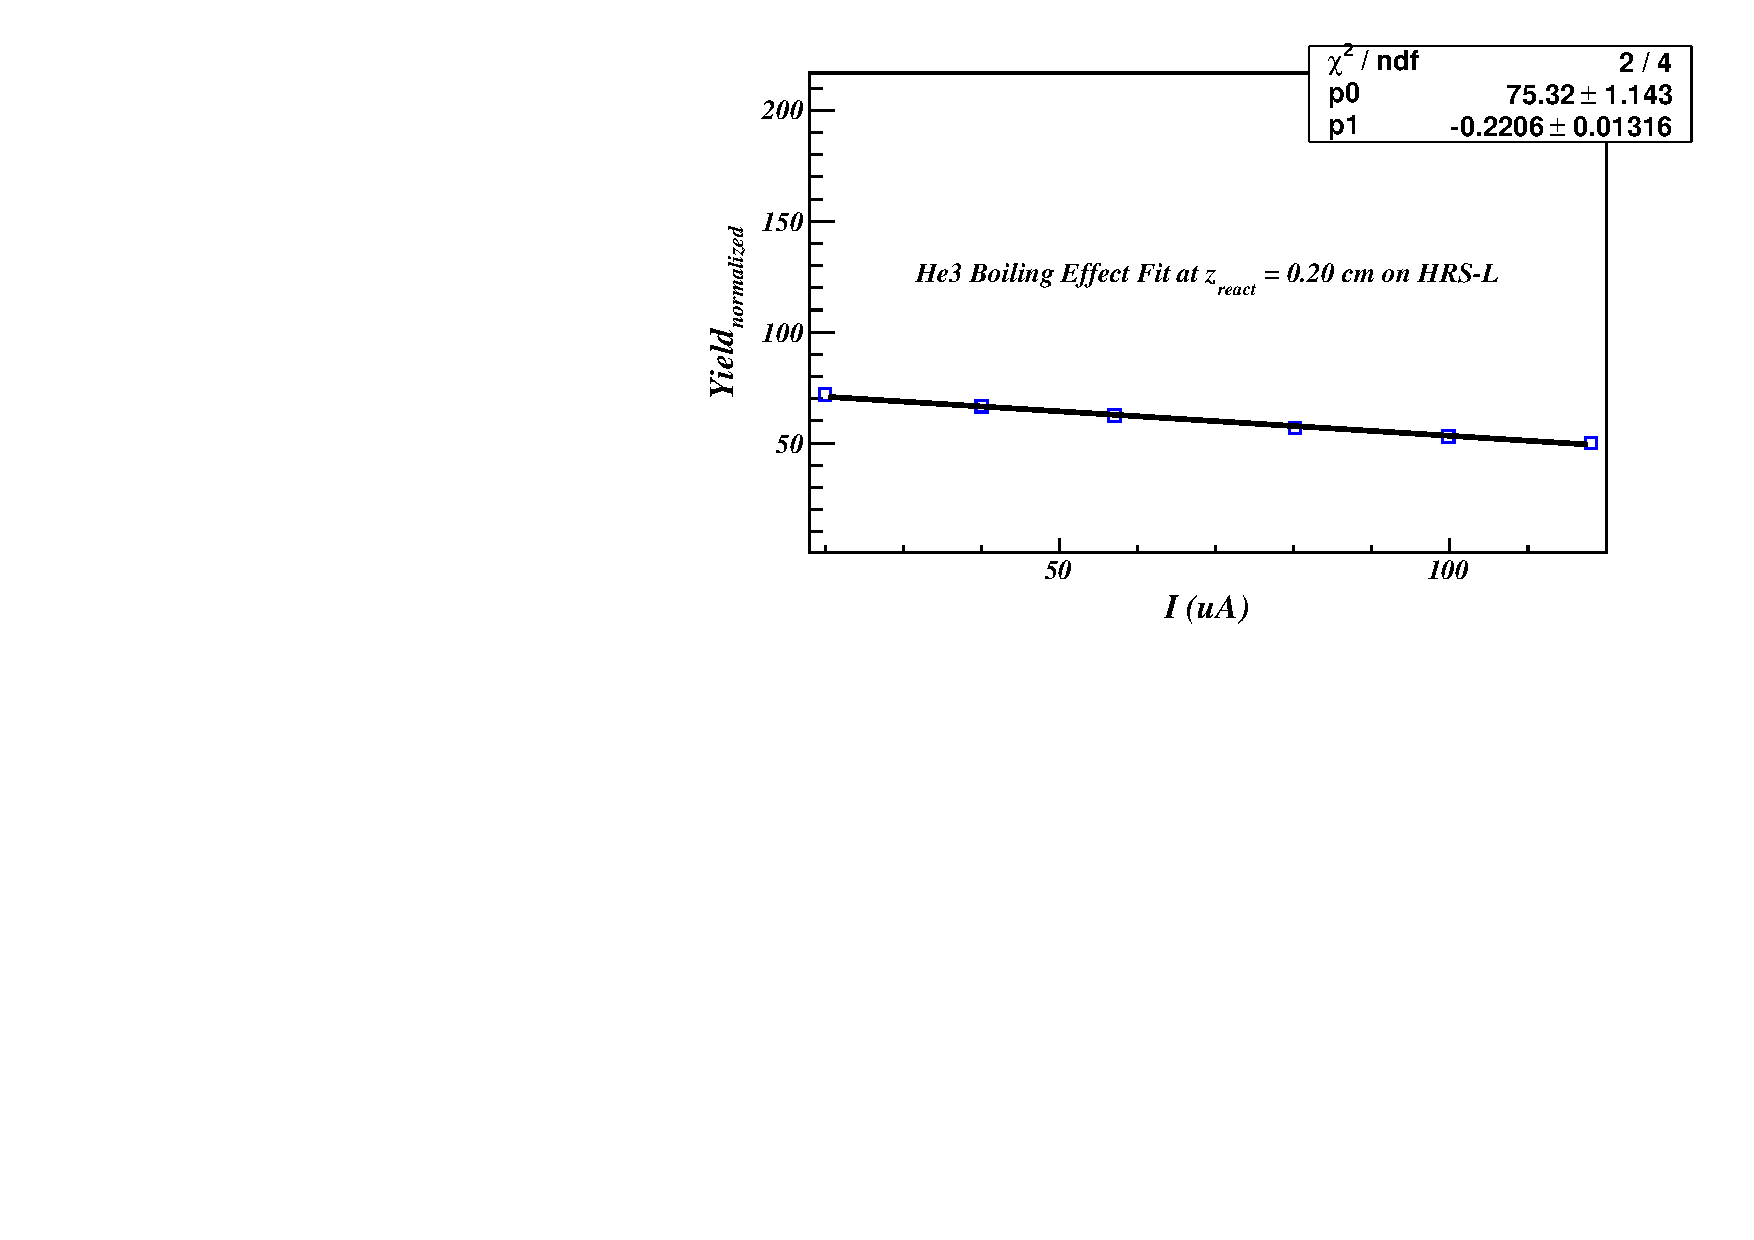
\includegraphics[type=pdf,ext=.pdf,read=.pdf,width=0.45\textwidth]{./figures/cryo/He3_Yield_L_All_0} 
    }
    \hfill
    \subfloat[$\mathrm{^{3}He}$ on HRS-R]{
      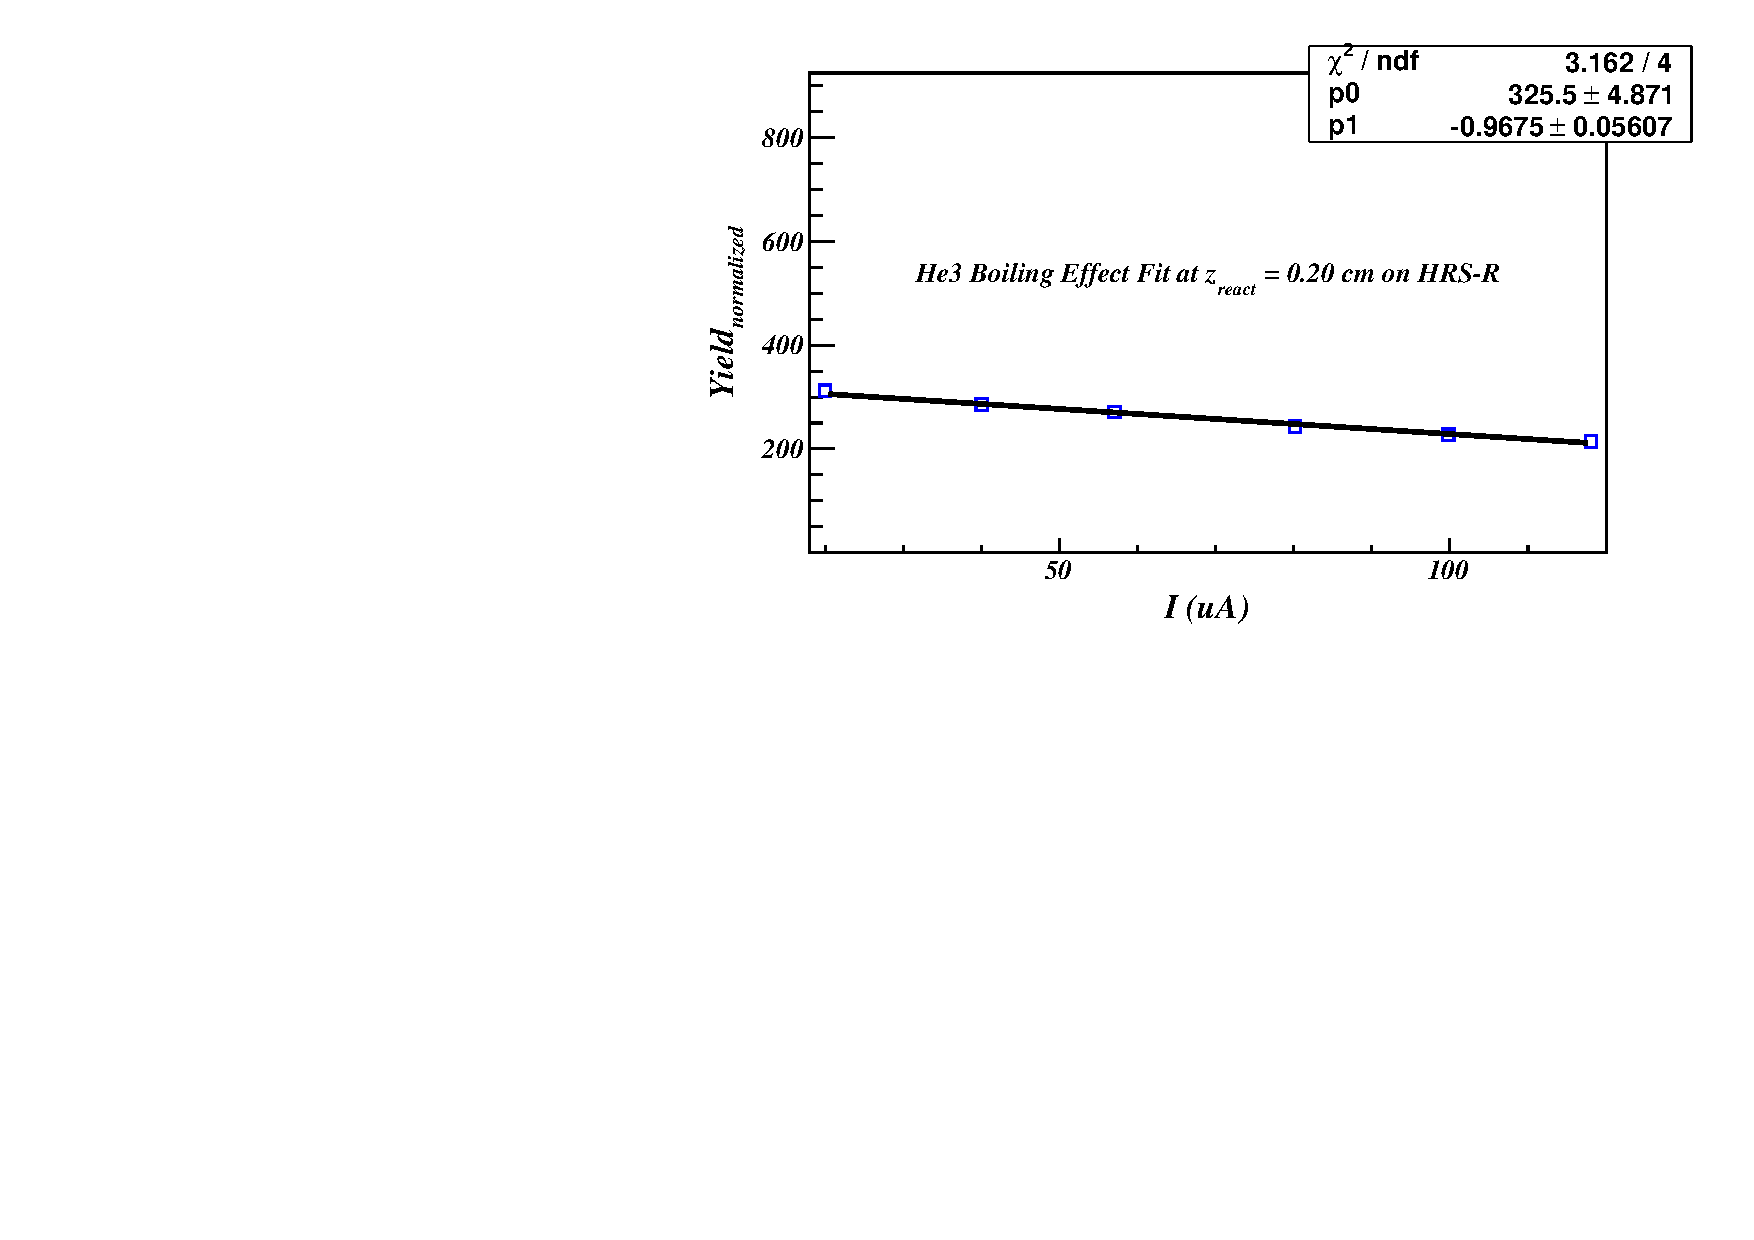
\includegraphics[type=pdf,ext=.pdf,read=.pdf,width=0.45\textwidth]{./figures/cryo/He3_Yield_R_All_0} 
    }
\\
    \subfloat[$\mathrm{^{4}He}$ on HRS-L]{
      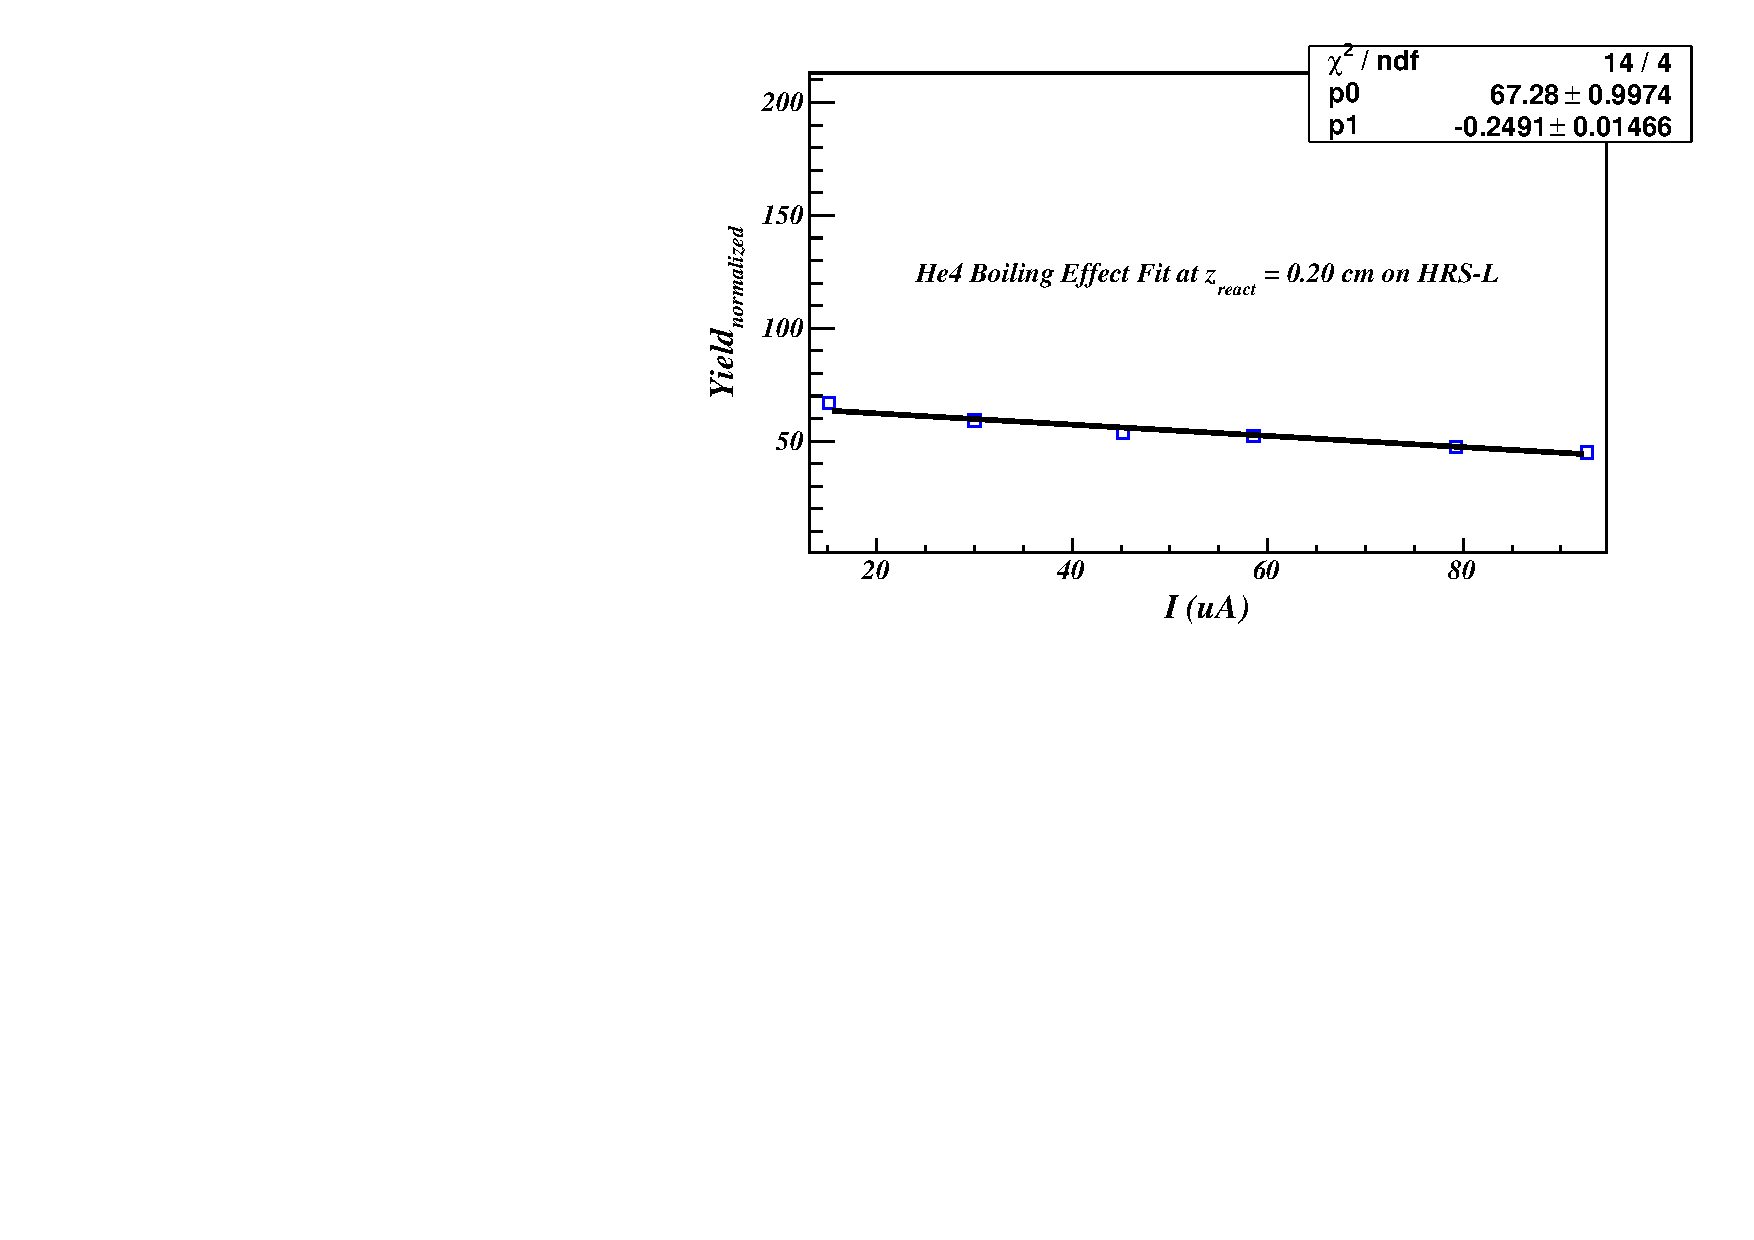
\includegraphics[type=pdf,ext=.pdf,read=.pdf,width=0.45\textwidth]{./figures/cryo/He4_Yield_L_All_0} 
    }
    \hfill
    \subfloat[$\mathrm{^{4}He}$ on HRS-R]{
      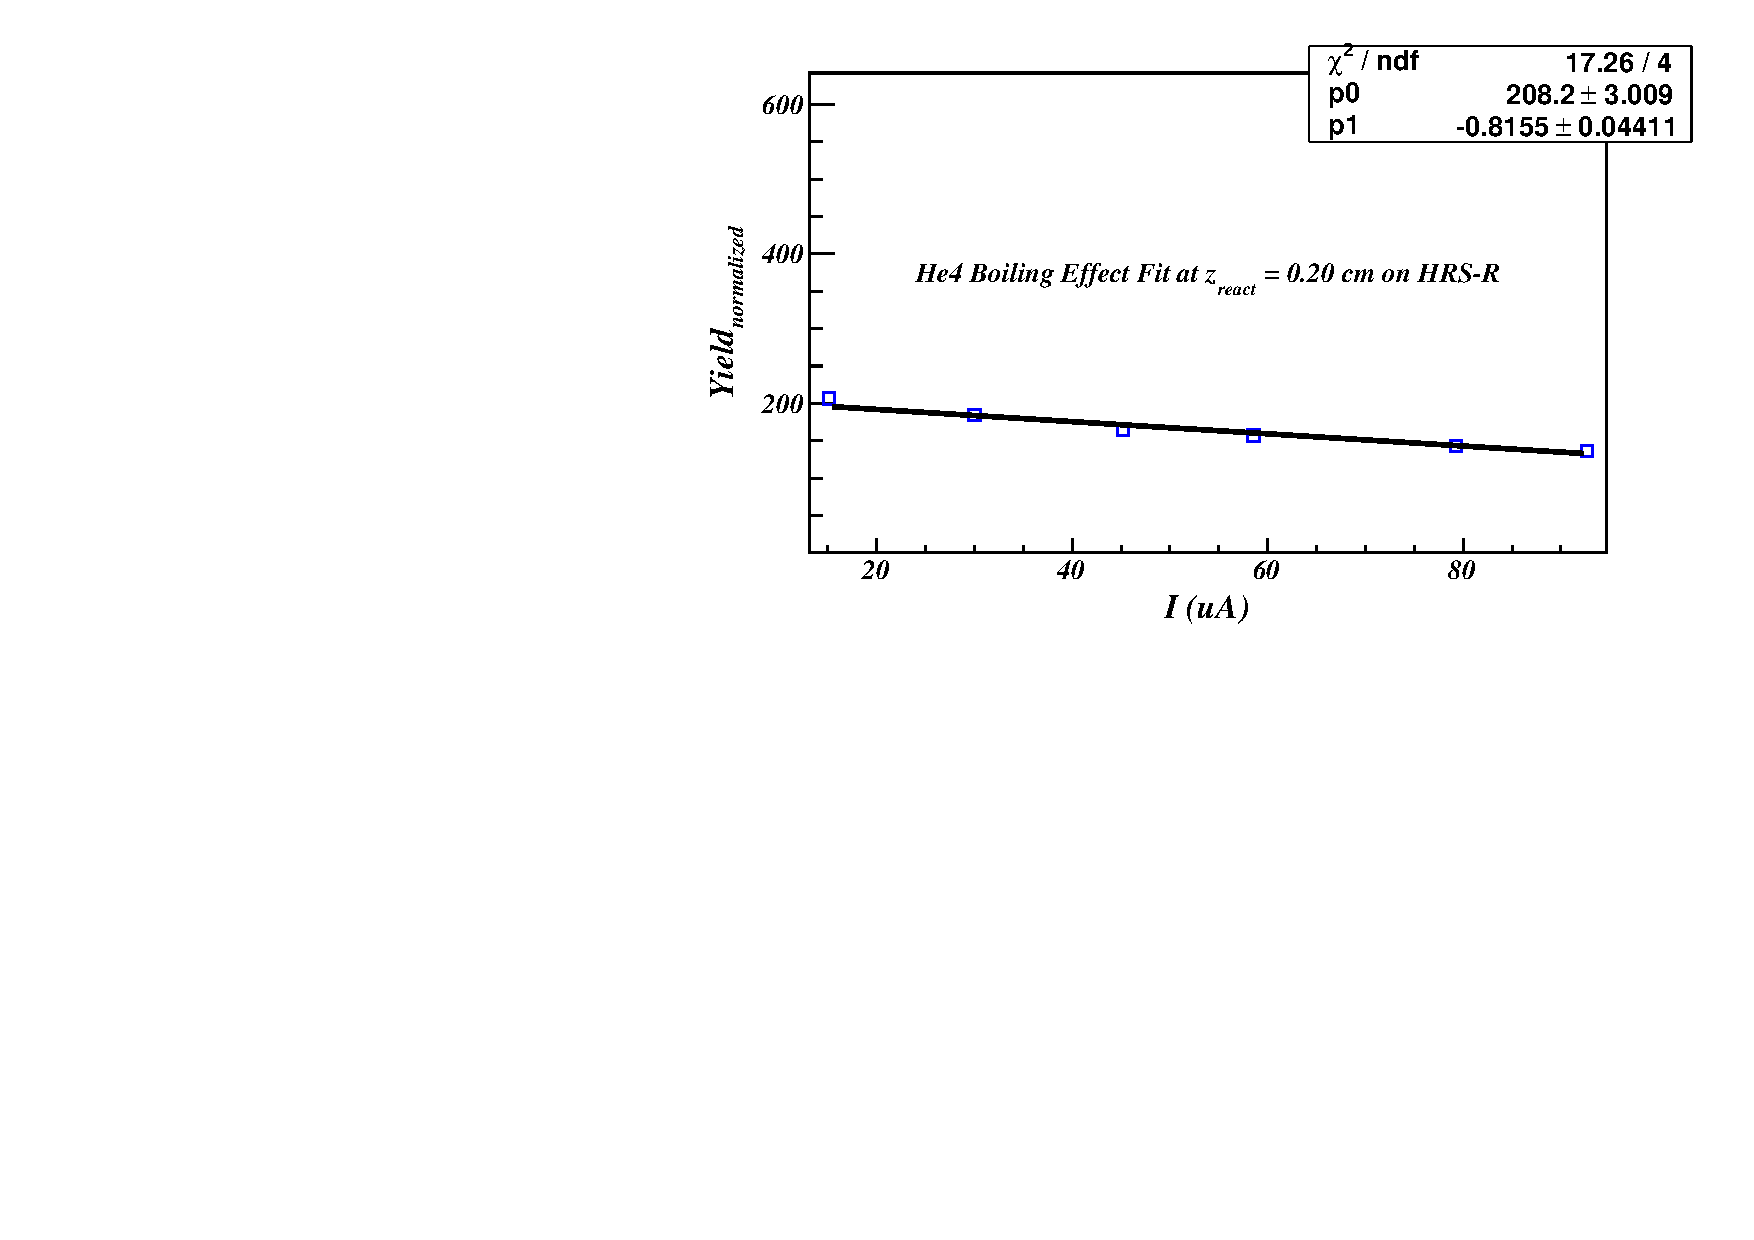
\includegraphics[type=pdf,ext=.pdf,read=.pdf,width=0.45\textwidth]{./figures/cryo/He4_Yield_R_All_0} 
    }
    \caption[Cryo-targets boiling effect fitting]{\footnotesize{Cryo-targets boiling effect fitting. They are examples near the center of the targets. Each target was divided into 60 bins along the target cell, where the boiling factor was individually fitted. The yield values have been normalized by a common factor.}}
    \label{cryo_boil_fit}
  \end{center}
\end{figure}
\begin{figure}[!h]
  \begin{center}
    \subfloat[$\mathrm{^{2}H2}$]{
      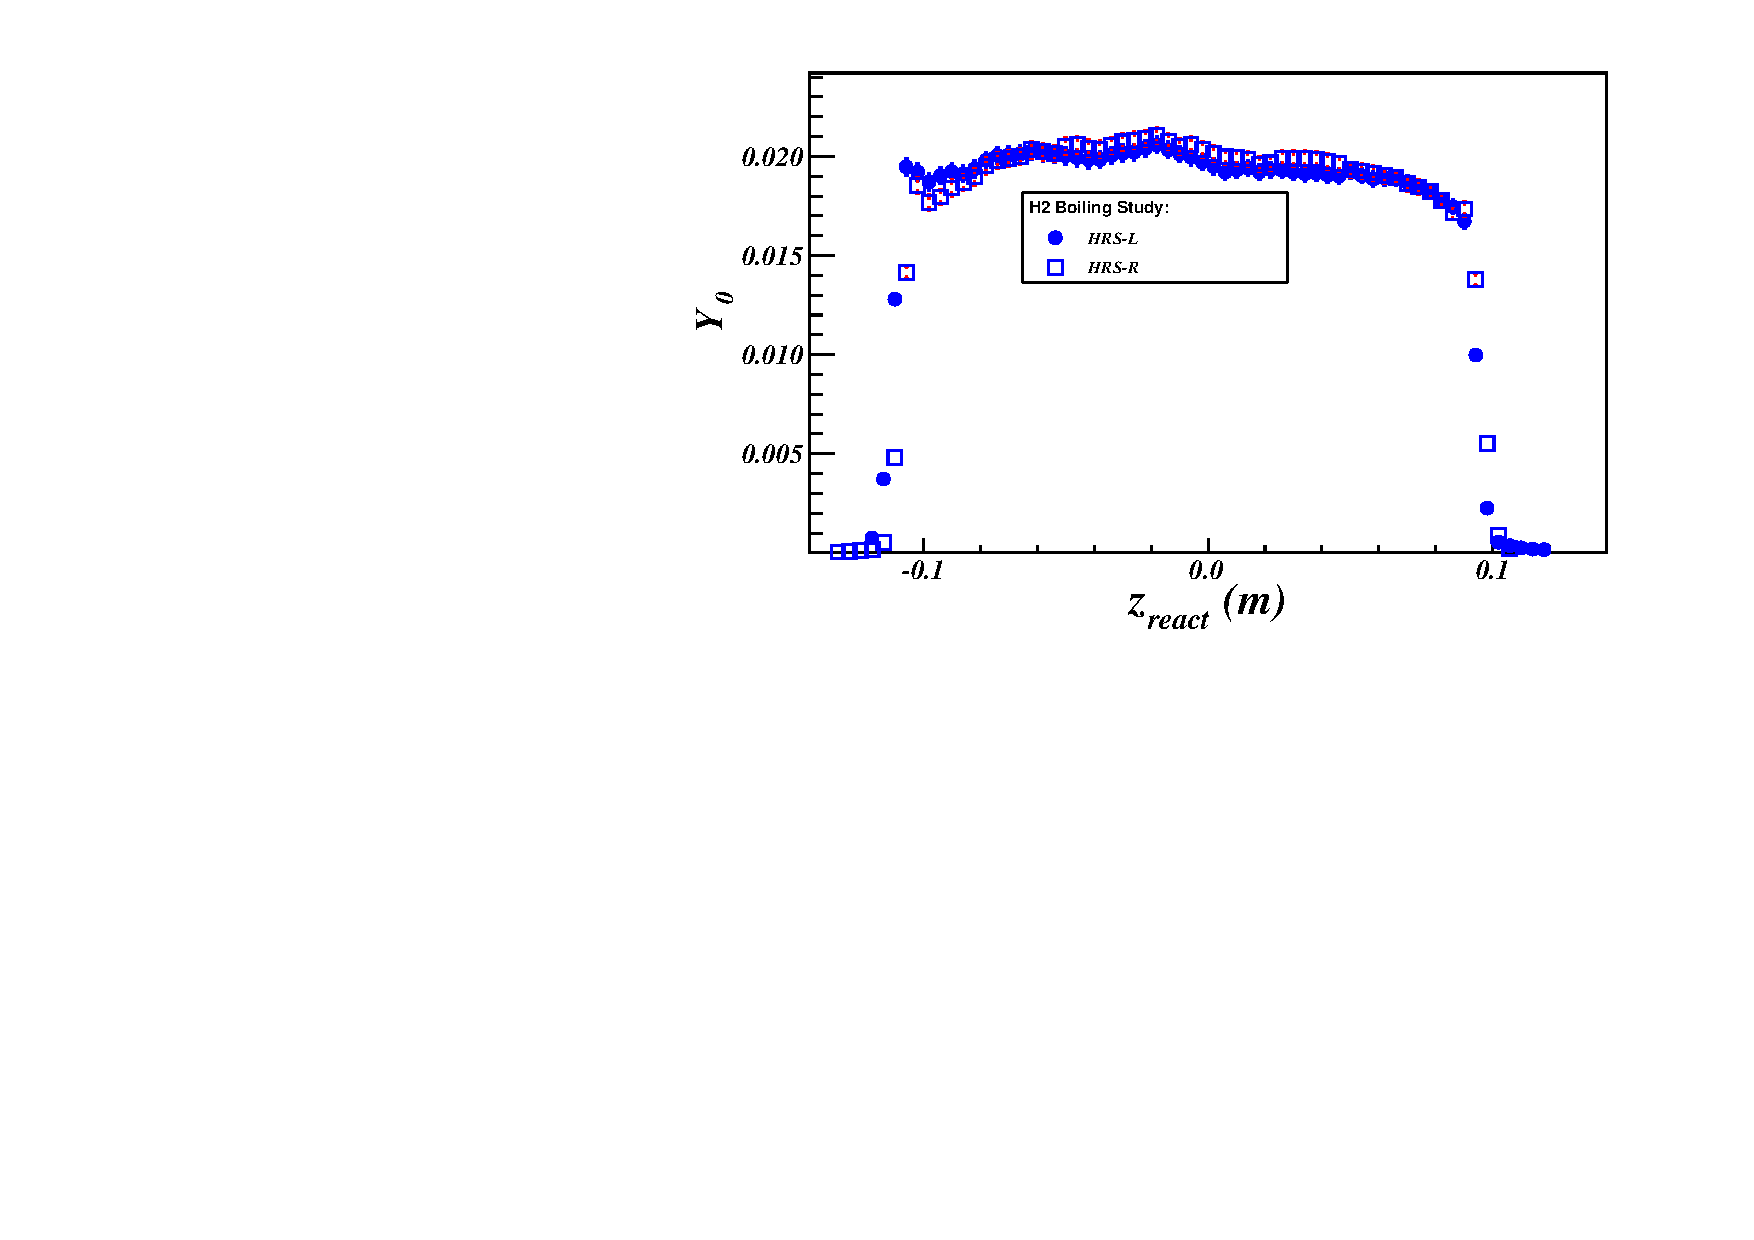
\includegraphics[type=pdf,ext=.pdf,read=.pdf,width=0.7\textwidth]{./figures/cryo/H2_Const} 
    }
    \hfill
    \subfloat[$\mathrm{^{3}He}$]{
      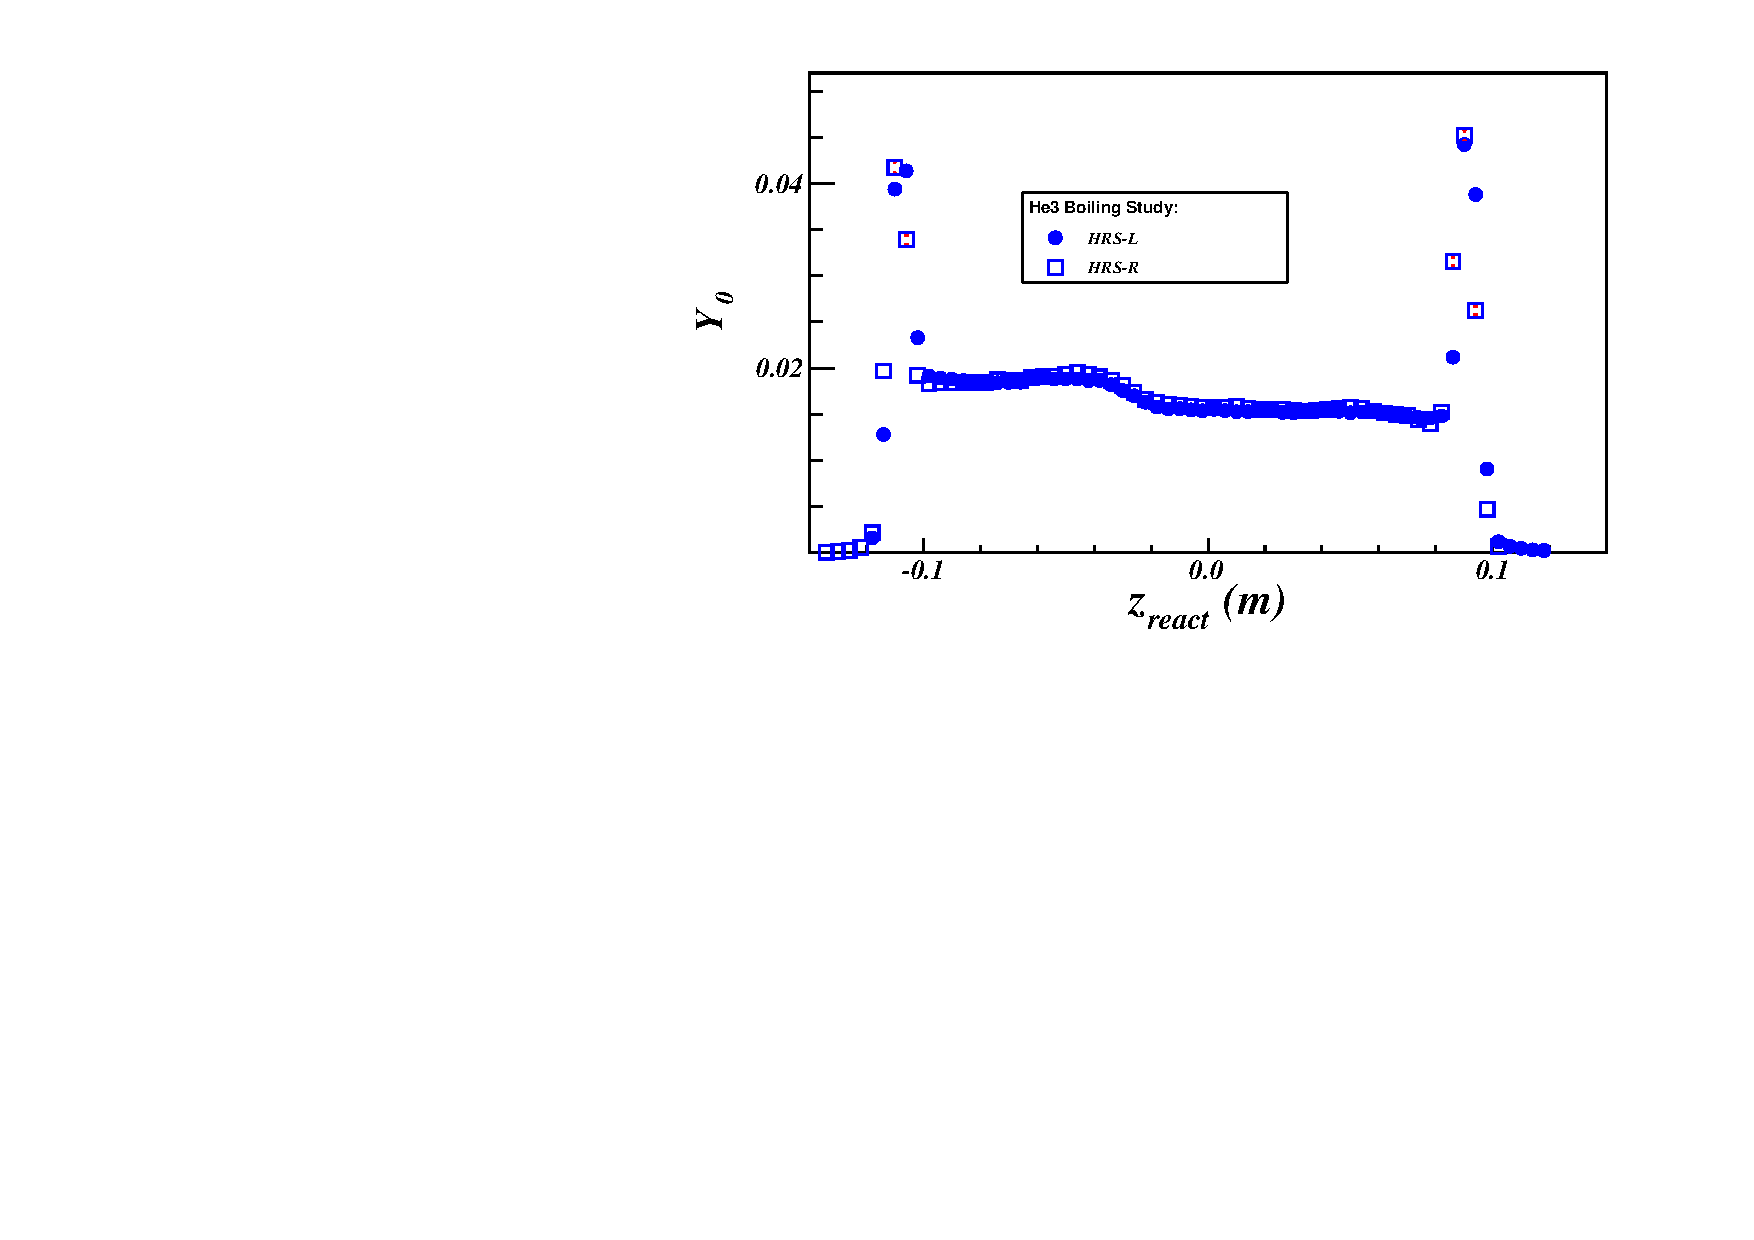
\includegraphics[type=pdf,ext=.pdf,read=.pdf,width=0.7\textwidth]{./figures/cryo/He3_Const} 
    }
     \hfill
    \subfloat[$\mathrm{^{4}He}$]{
      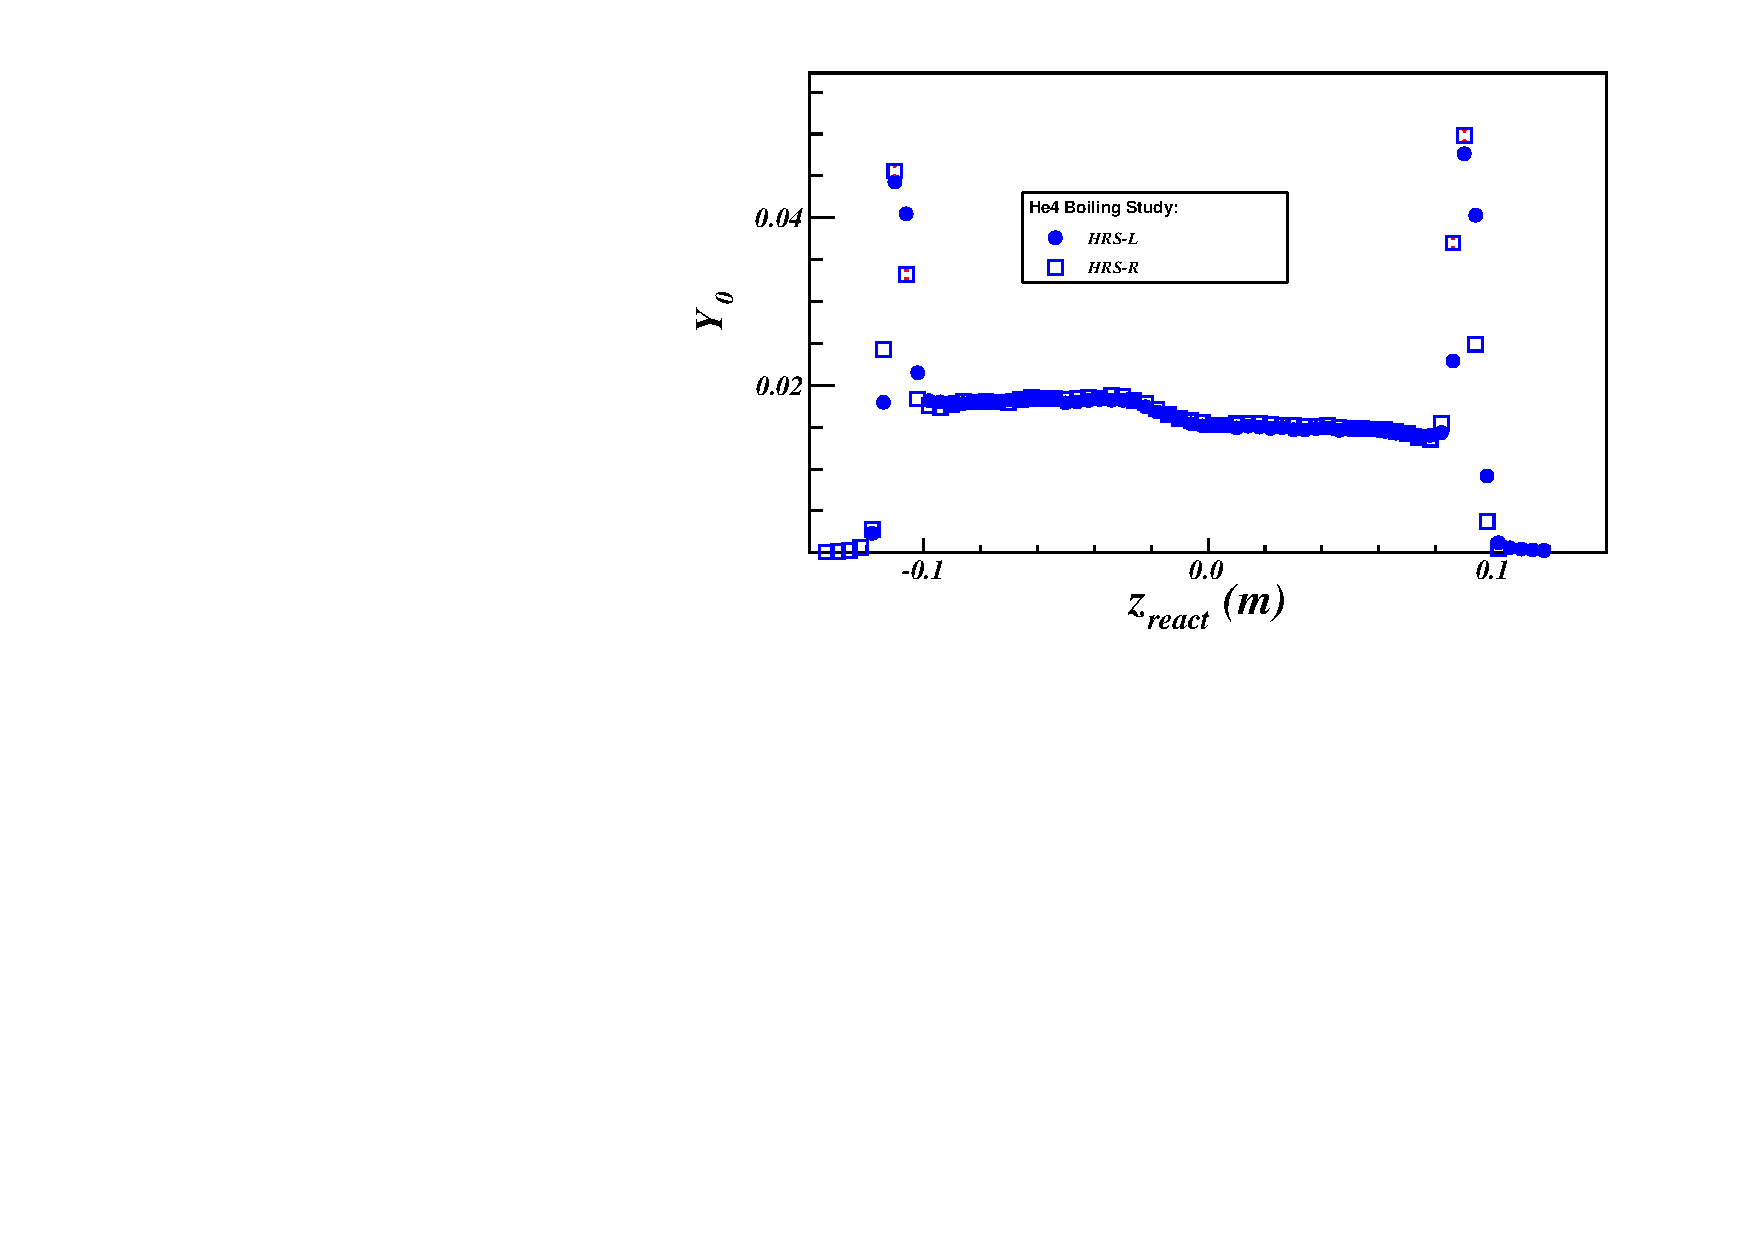
\includegraphics[type=pdf,ext=.pdf,read=.pdf,width=0.7\textwidth]{./figures/cryo/He4_Const} 
    }
    \caption[Cryo-target density profiles from the boiling study]{\footnotesize{Cryo-target density profiles from the boiling study. The results from both HRSs agree with each other for each target, and the peaks denote the contributions from the endcaps of the target cell.}}
    \label{cryo_boil_y0}
  \end{center}
\end{figure}

 Shown in Fig.~\ref{c12_boil_fit}, the fitting result of $\mathrm{^{12}C}$ indicates that for a fixed target density, the yield does not change at different current. For cryo-target, the data was binned in $z_{react}$ which was divided into 60 bins. In each bin, the yield was calculated and one can fit the boiling factor by the formula:
 \begin{equation}
  Y(I, z_{react}^{i}) = Y(0, z_{react}^{i}) + m(z_{react}^{i})\cdot I,,\quad where~i=1,\cdots,60,
  \label{eq_yield_rho_zbin}
\end{equation}
which gives the variation of the density in each bin:
 \begin{equation}
  \rho(I, z_{react}^{i}) = \rho(0, z_{react}^{i}) \cdot (1.0 + BF(z_{react}^{i}) \cdot I /100),
  \label{eq_rho_zbin}
 \end{equation}
where,
 \begin{equation}
   BF(z_{react}^{i})=\frac{Y(0, z_{react}^{i})}{m(z_{react}^{i})}. \\
     \label{eq_bf_zbin}
 \end{equation}

As examples, Fig.~\ref{cryo_boil_fit} shows the fitting results of boiling factors at the center of $z_{react}$ for three cryo-targets, where the curves are well fitted by linear functions. The curve of normalized $Y(0, z_{react}^{i})$ denotes the target density profile along the cell, as shown in Fig.~\ref{cryo_boil_y0}, where the peaks of endcaps can be clearly seen. The distribution of $BF(z_{react}^{i})$ for each target, given in Fig.~\ref{cryo_boil_fact}, shows the boiling effects at different $z_{react}$, and demonstrates that the non-uniform cryo-target densities were mainly caused by the highly localized boiling effects. In the plot, the values of $z_{react}$ at the positions of endcaps are close to zero which agree with the fact that the density of aluminium walls shouldn't change with beam current. Results from both HRSs were compared and found out to agree nicely with each other. 
 \begin{figure}[]
  \begin{center}
    \subfloat[$\mathrm{^{2}H}$]{
      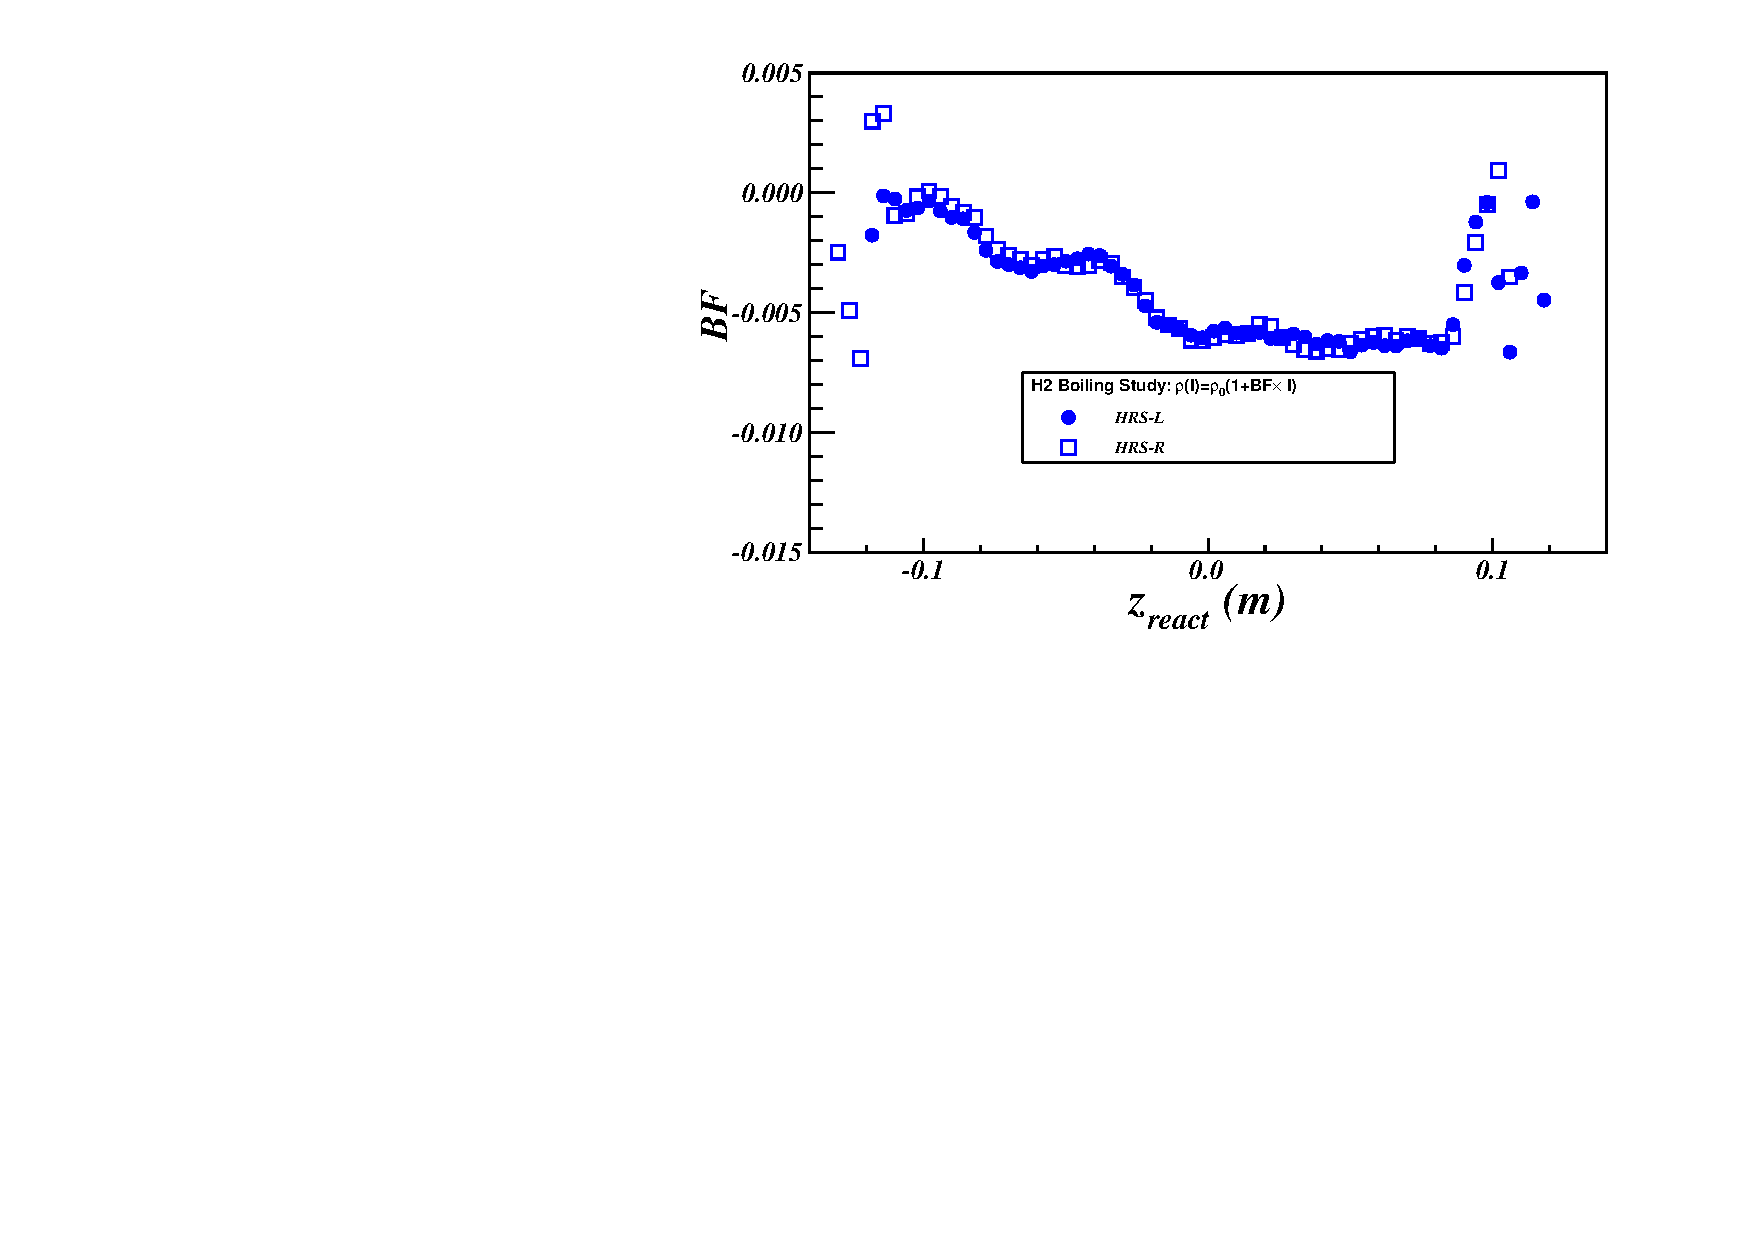
\includegraphics[type=pdf,ext=.pdf,read=.pdf,width=0.7\textwidth]{./figures/cryo/H2_BF} 
    }
    \hfill
    \subfloat[$\mathrm{^{3}He}$]{
      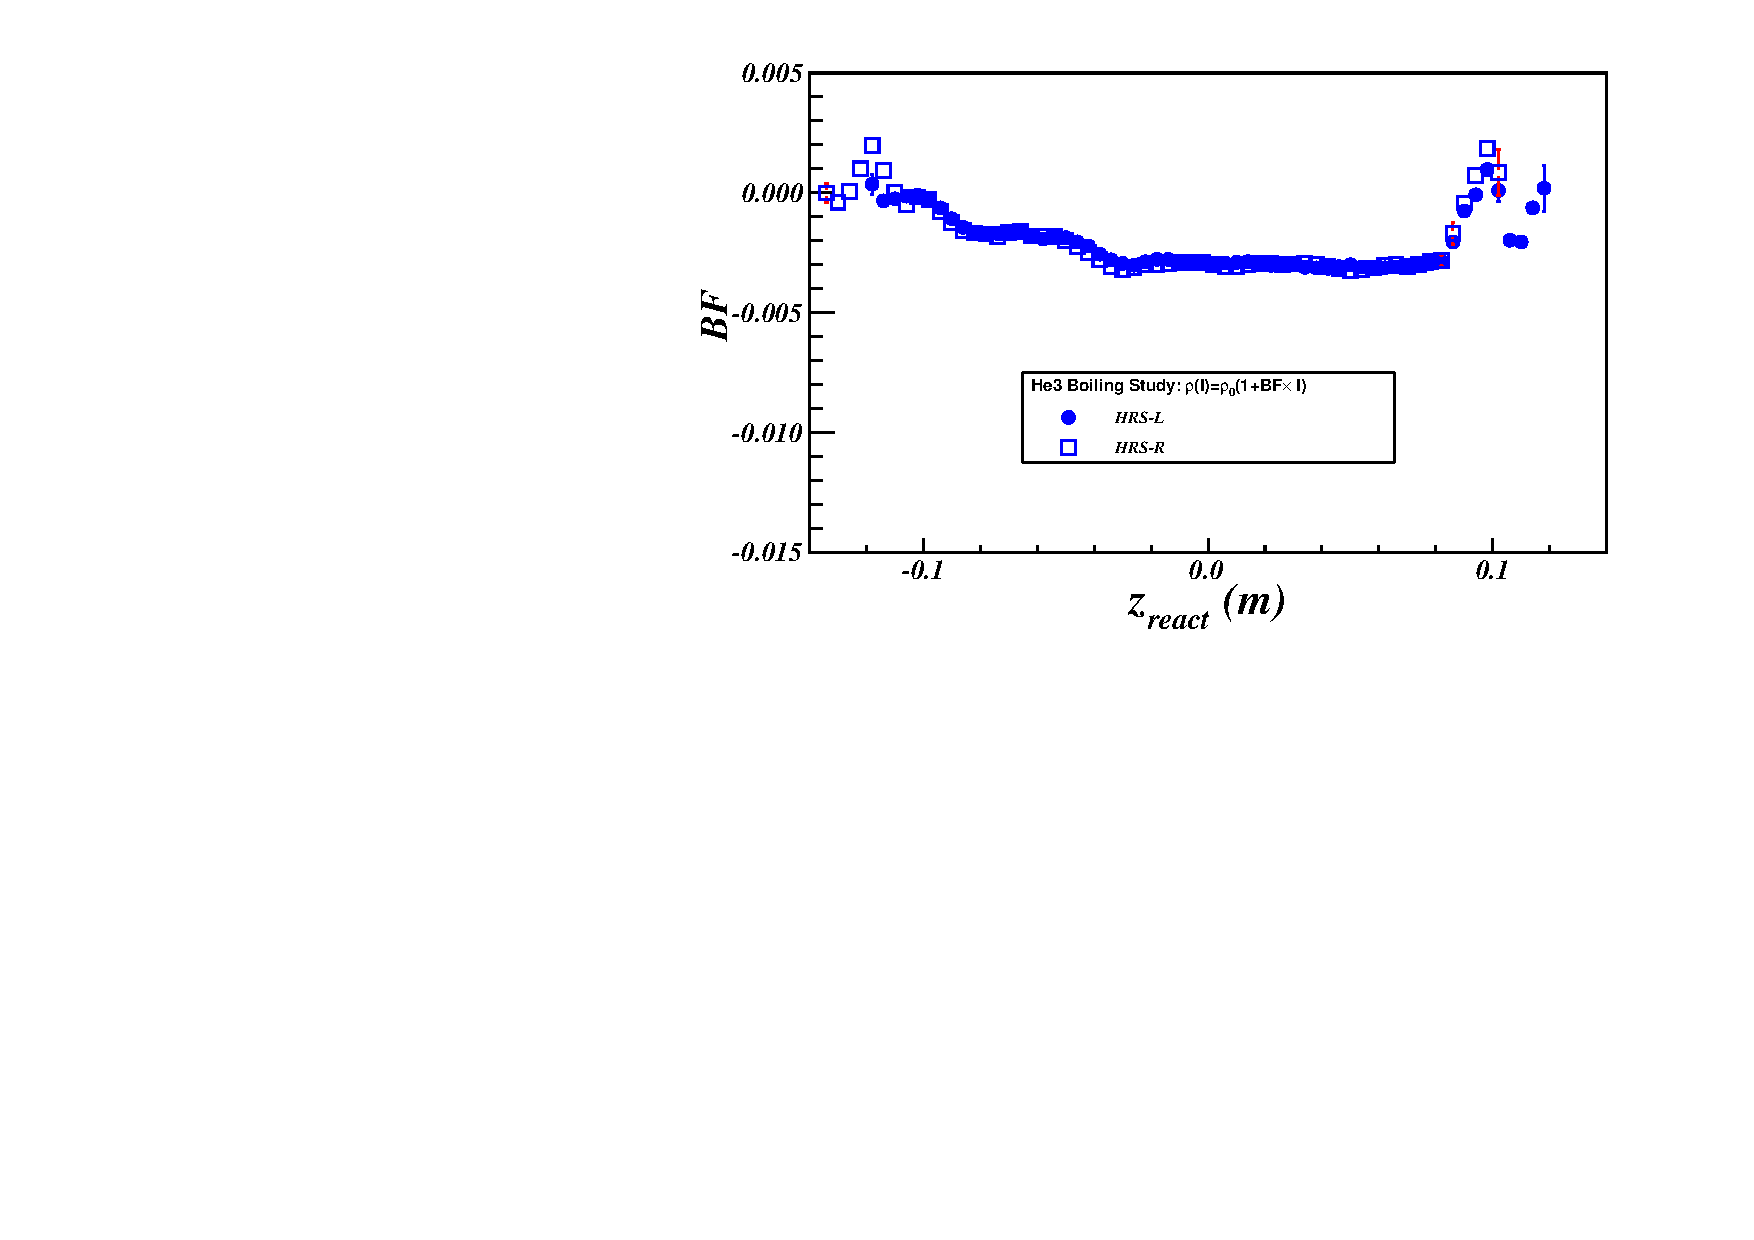
\includegraphics[type=pdf,ext=.pdf,read=.pdf,width=0.7\textwidth]{./figures/cryo/He3_BF} 
    }
     \hfill
    \subfloat[$\mathrm{^{4}He}$]{
      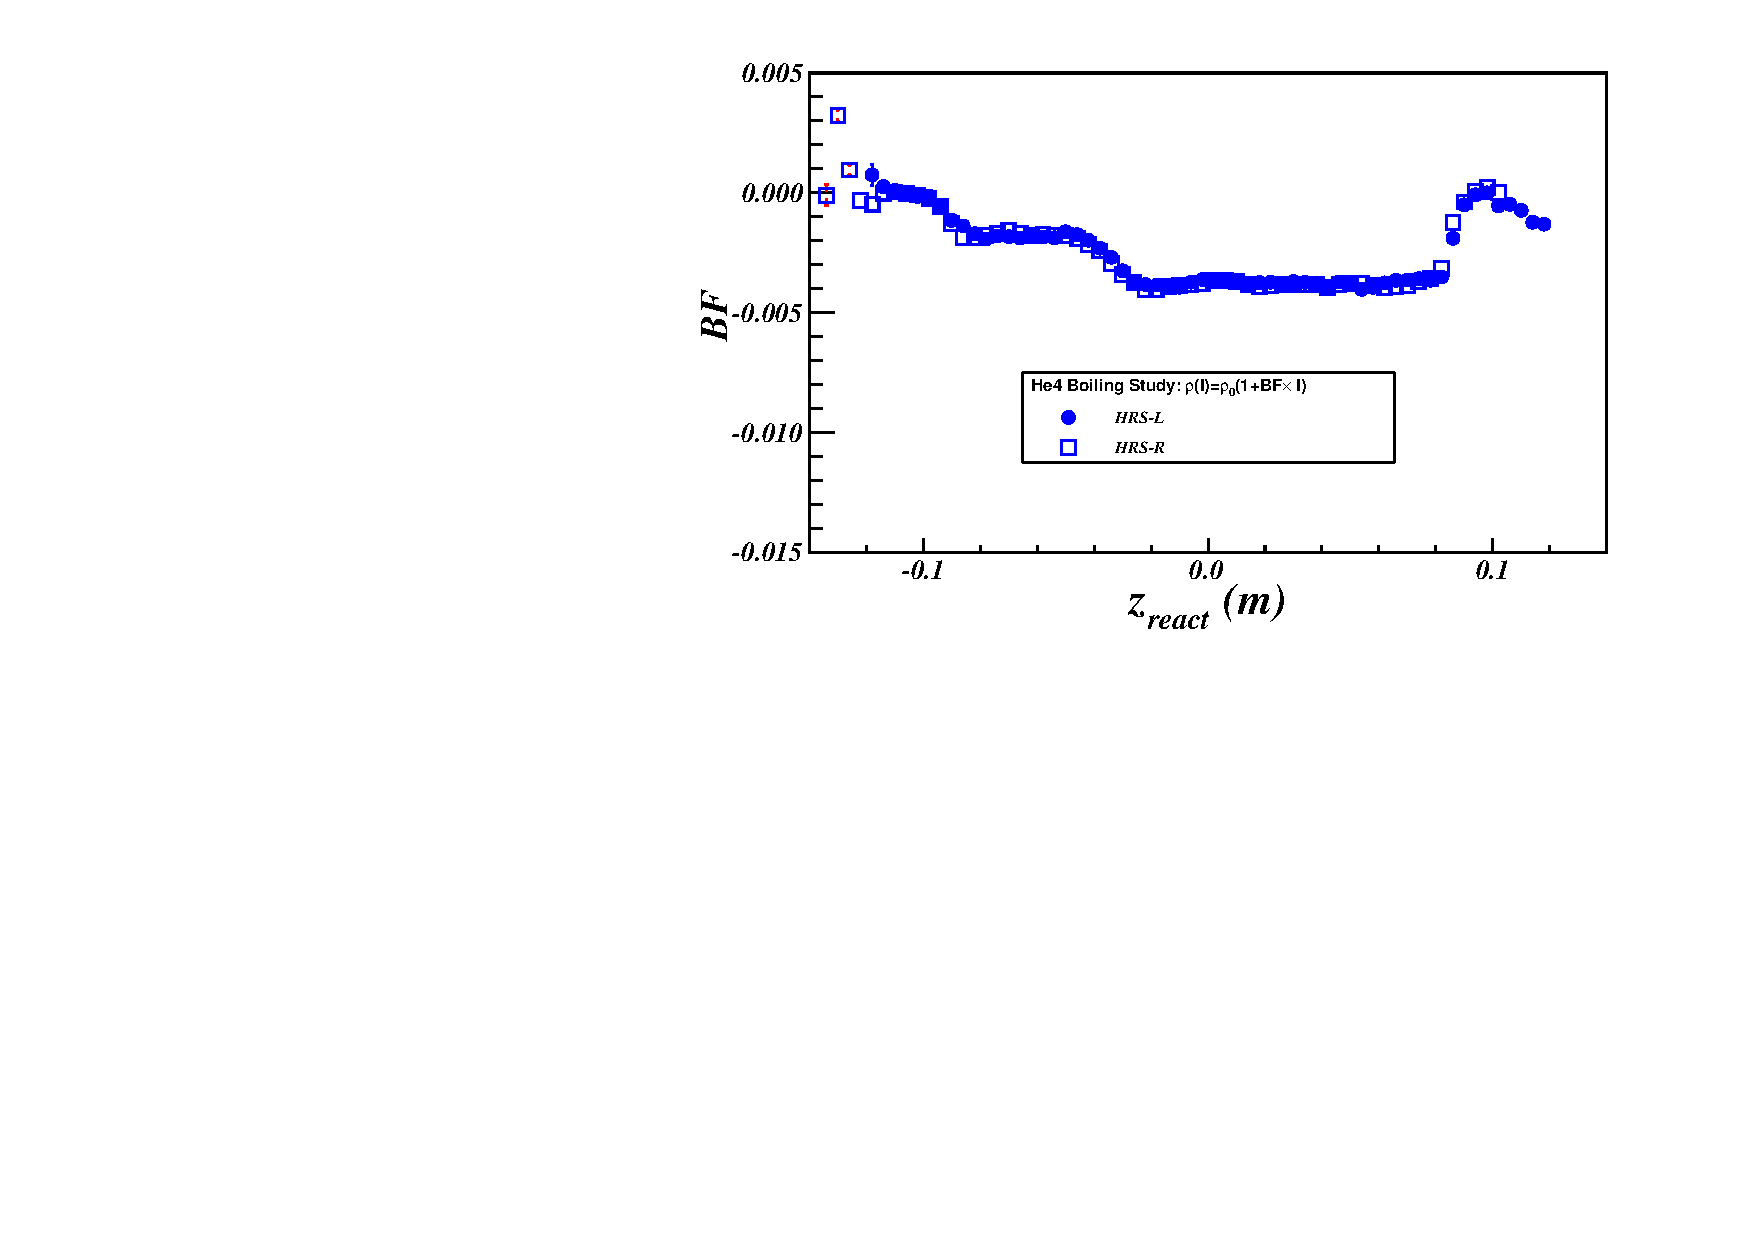
\includegraphics[type=pdf,ext=.pdf,read=.pdf,width=0.7\textwidth]{./figures/cryo/He4_BF} 
    }
    \caption[Cryo-target boiling factor distribution]{\footnotesize{Cryo-target boiling factor distribution. Each plot clearly shows that the boiling effect varies along the target cells. The boiling factors at the endcaps are reasonably close to zero. The studies from both HRSs give consistent results. The yield values had been normalized by a common factor.}}
    \label{cryo_boil_fact}
  \end{center}
\end{figure}

\section{Extracting Density Distributions}
  From Eq.~\eqref{eq_yield_rho_zbin}, the target density profile can be obtained by extracting the distribution of $Y(0)$ during the boiling study. In this section, a different method is applied to extract the density distribution by with the experimental data and simulation data. 
  
  Since $z_{react}$ is along the incoming beam direction so as the orientation of the target cell, the $z_{react}$ distribution in the experimental data, $z_{react}^{EX}$, gives the distribution of yields in one current setting. Meanwhile, the yield for one $z_{react}^{EX}$ value is proportional to the density of the target in this location, so one expects to study the density distribution of the target with the $z_{react}^{EX}$ distribution. However, $z_{react}^{EX}$ should also contain the acceptance effect of the HRS and the cross section weighting effect. One can use the simulation data generated by SAMC which simulates the acceptance effect of HRSs, and plot the simulated $z_{react}$ distribution, $z_{react}^{MC}$. One can further weight $z_{react}^{MC}$ by the cross section values calculated from XEMC. When the target density distribution in the simulation data is uniform, $z_{react}^{MC}$ only carries the acceptance effect and the cross section effect. By plotting the histograms of $z_{react}^{EX}$ and $z_{react}^{MC}$ with the same range and bin-size, one takes to ratio of two histogram, which leads to a clean relative density distribution of the target at the current setting.
  
   The plots on the left hand side of Fig.~\ref{cryo_den_fit} show the distribution of $z_{react}^{EX}$ and $z_{react}^{MC}$ at three different current settings for each target, while the plots on the right hand side give the fitting results of the relative density distributions. A polynomial function is used for each fitting process. 
 \begin{figure}[!ht]
  \begin{center}
    \subfloat[$\mathrm{^{2}H}$]{
      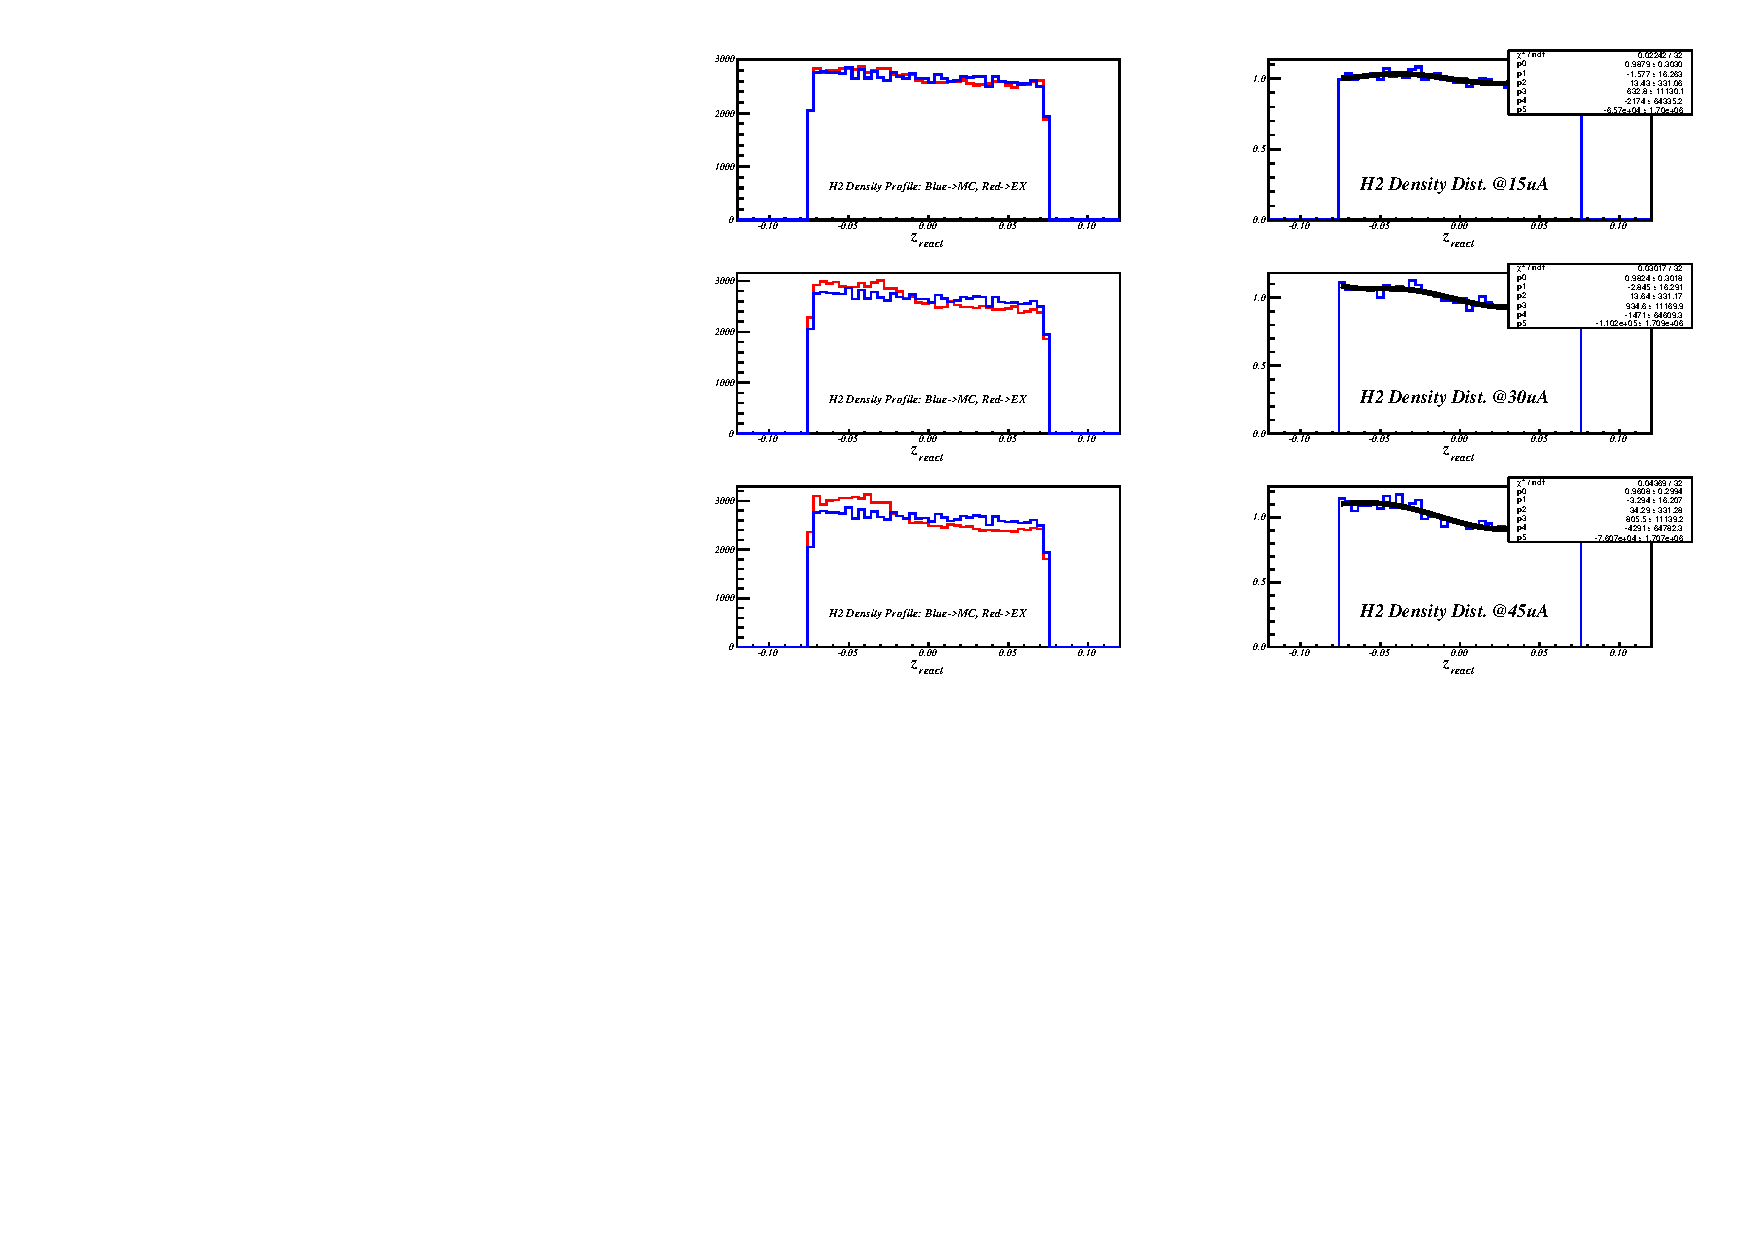
\includegraphics[type=pdf,ext=.pdf,read=.pdf,width=0.7\textwidth]{./figures/cryo/H2_Boiling_Density} 
    }
    \hfill
    \subfloat[$\mathrm{^{3}He}$]{
      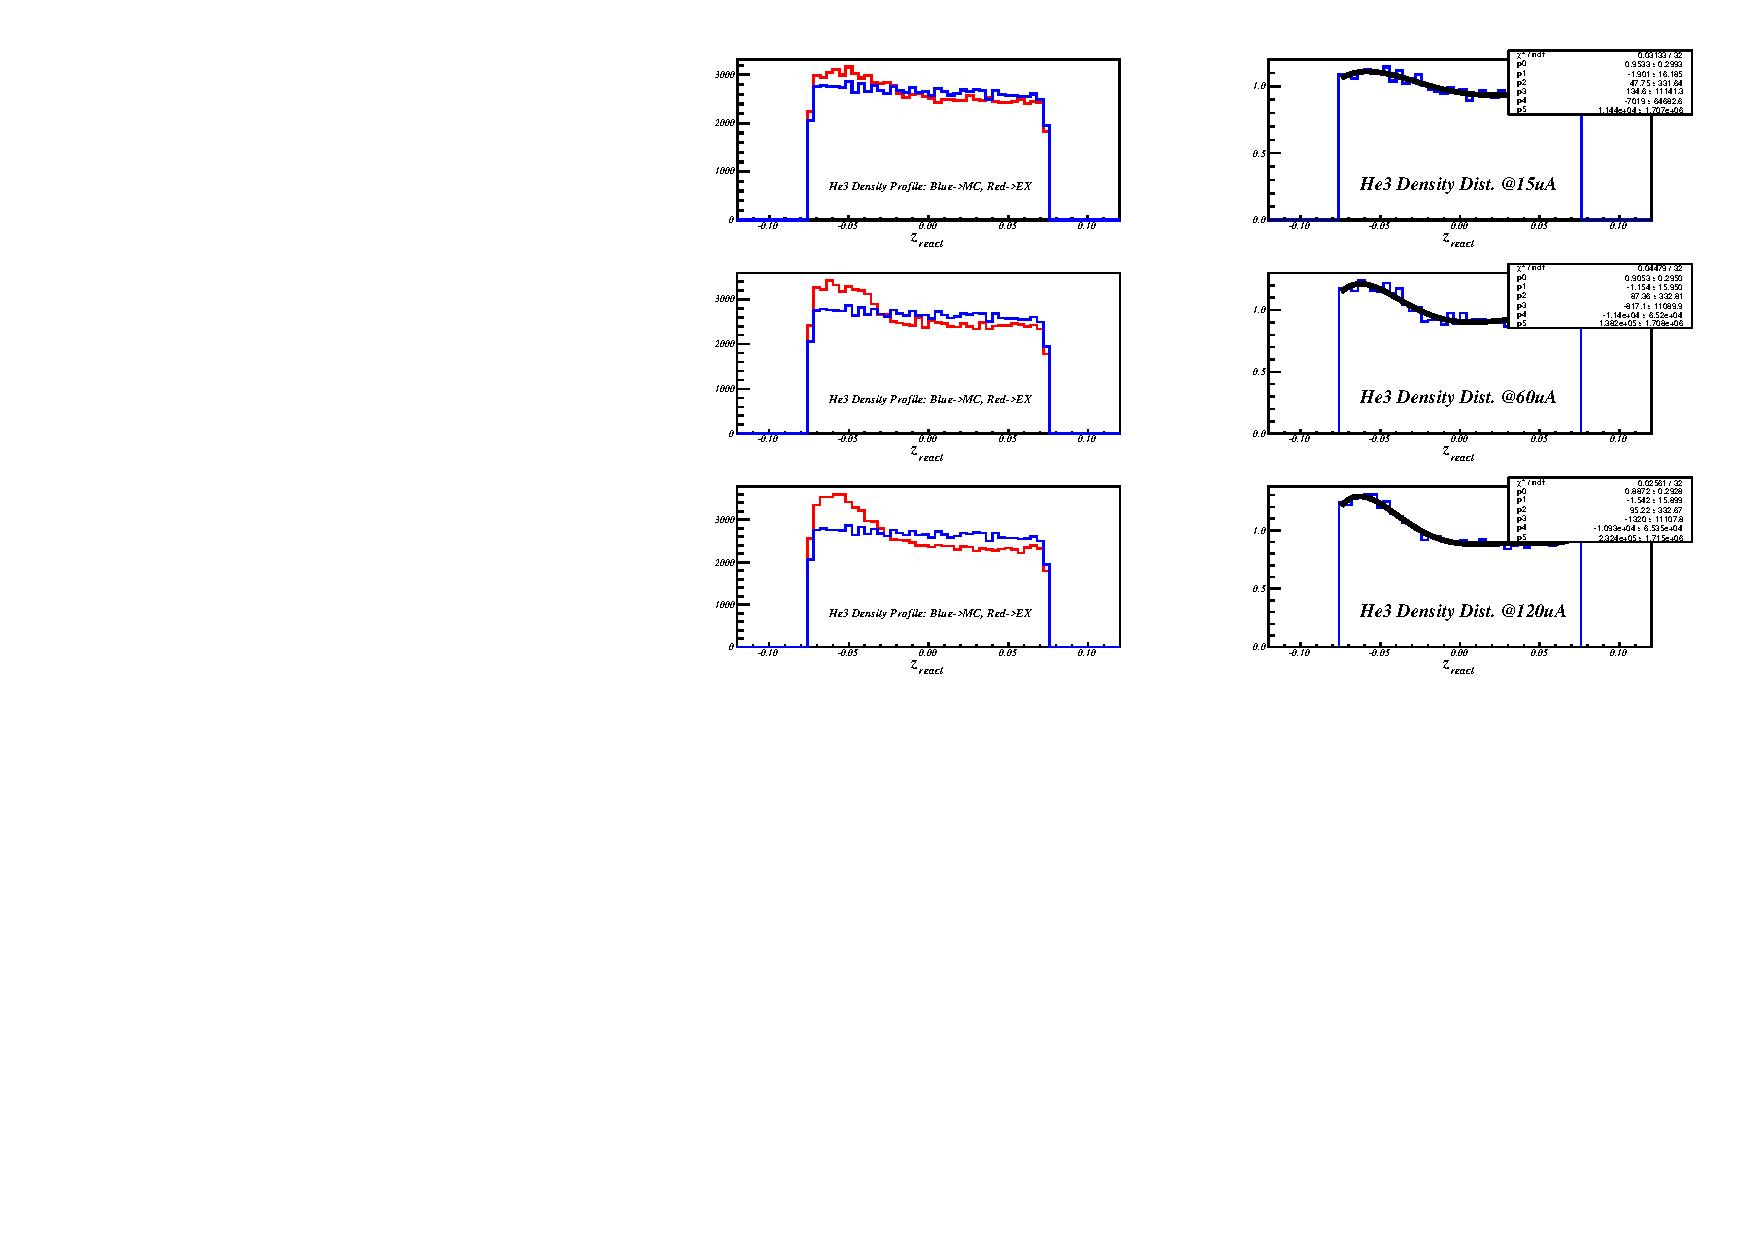
\includegraphics[type=pdf,ext=.pdf,read=.pdf,width=0.7\textwidth]{./figures/cryo/He3_Boiling_Density} 
    }
     \hfill
    \subfloat[$\mathrm{^{4}He}$]{
      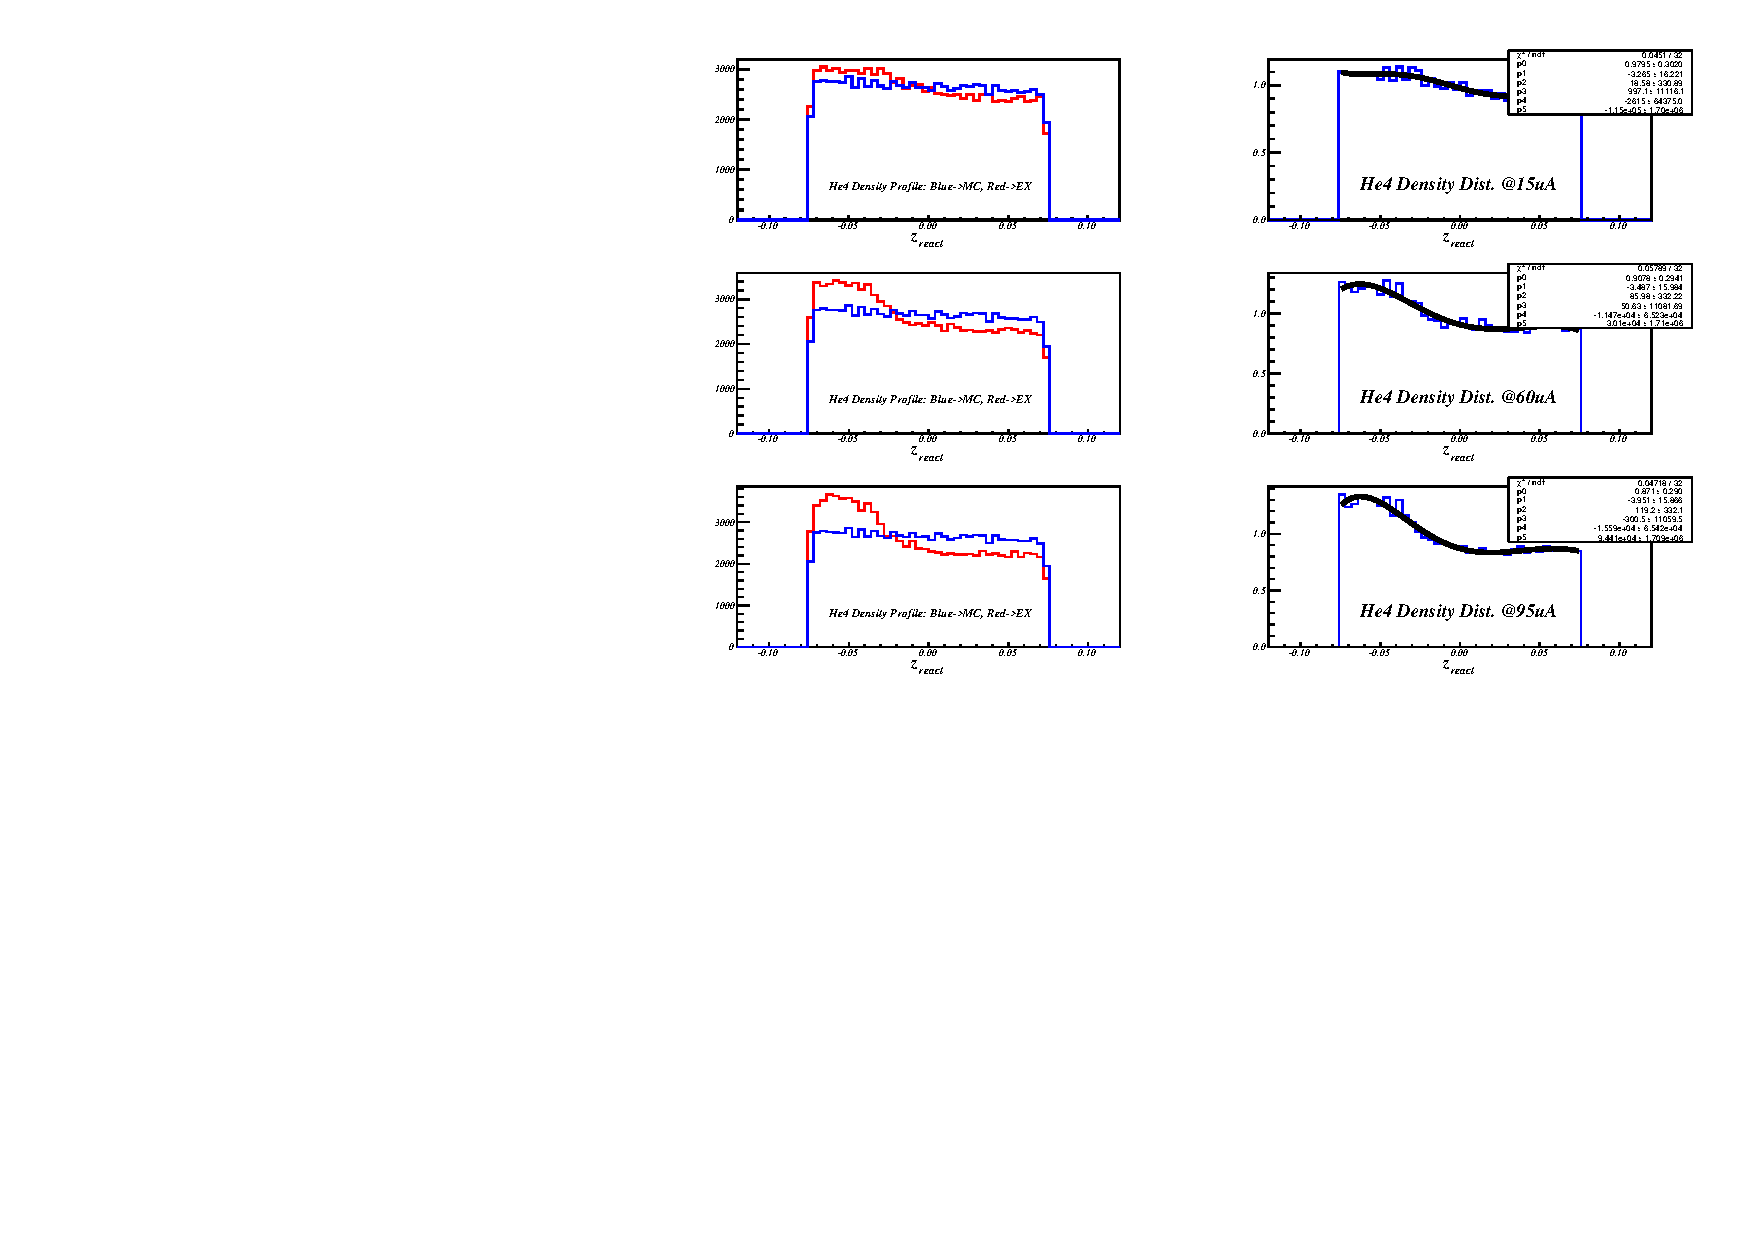
\includegraphics[type=pdf,ext=.pdf,read=.pdf,width=0.7\textwidth]{./figures/cryo/He4_Boiling_Density} 
    }
    \caption[Cryo-target density distributions extracted from data]{\footnotesize{Cryo-target density distributions extracted from data. The density distribution was extracted by taking the histogram ratio of $z_{react}$ from experimental data (red lines in plots on the left panel) and from simulation data with flat density distribution (blue lines in plots on the left panel). For each target, the density distributions at the minimum, middle and maximum currents were individually extracted (on right panel). The current settings are given in the plots.}}
    \label{cryo_den_fit}
  \end{center}
\end{figure}

 One can use the density distributions at the minimum current (15 uA, 20 uA and 15 uA for $\mathrm{^{2}H}$, $\mathrm{^{3}He}$ and $\mathrm{^{4}He}$, respectively), and apply the boiling factors to calculate the density distribution at beam current equal to zero, $\rho(0)$. Then the density distribution at any current settings, $\rho_{Calc}(I)$ can be calculated with Eq.~\eqref{eq_rho_zbin}. To verify the boiling study results and the density distributions at different current settings, the distributions of $\rho_{Calc}(I)$ and $\rho(I)$ extracted in Fig.~\ref{cryo_den_fit} were compared, as shown in Fig.~\ref{cryo_den_comp}. Note that the contributions from the two endcaps were removed by applying the cut, $|z_{react}|\leq 7.5~cm$. The plots reveal that the results of boiling study successfully characterize the change of target density with different beam currents.
  \begin{figure}[!ht]
  \begin{center}
    \subfloat[$\mathrm{^{2}H}$ at I=30 uA]{
      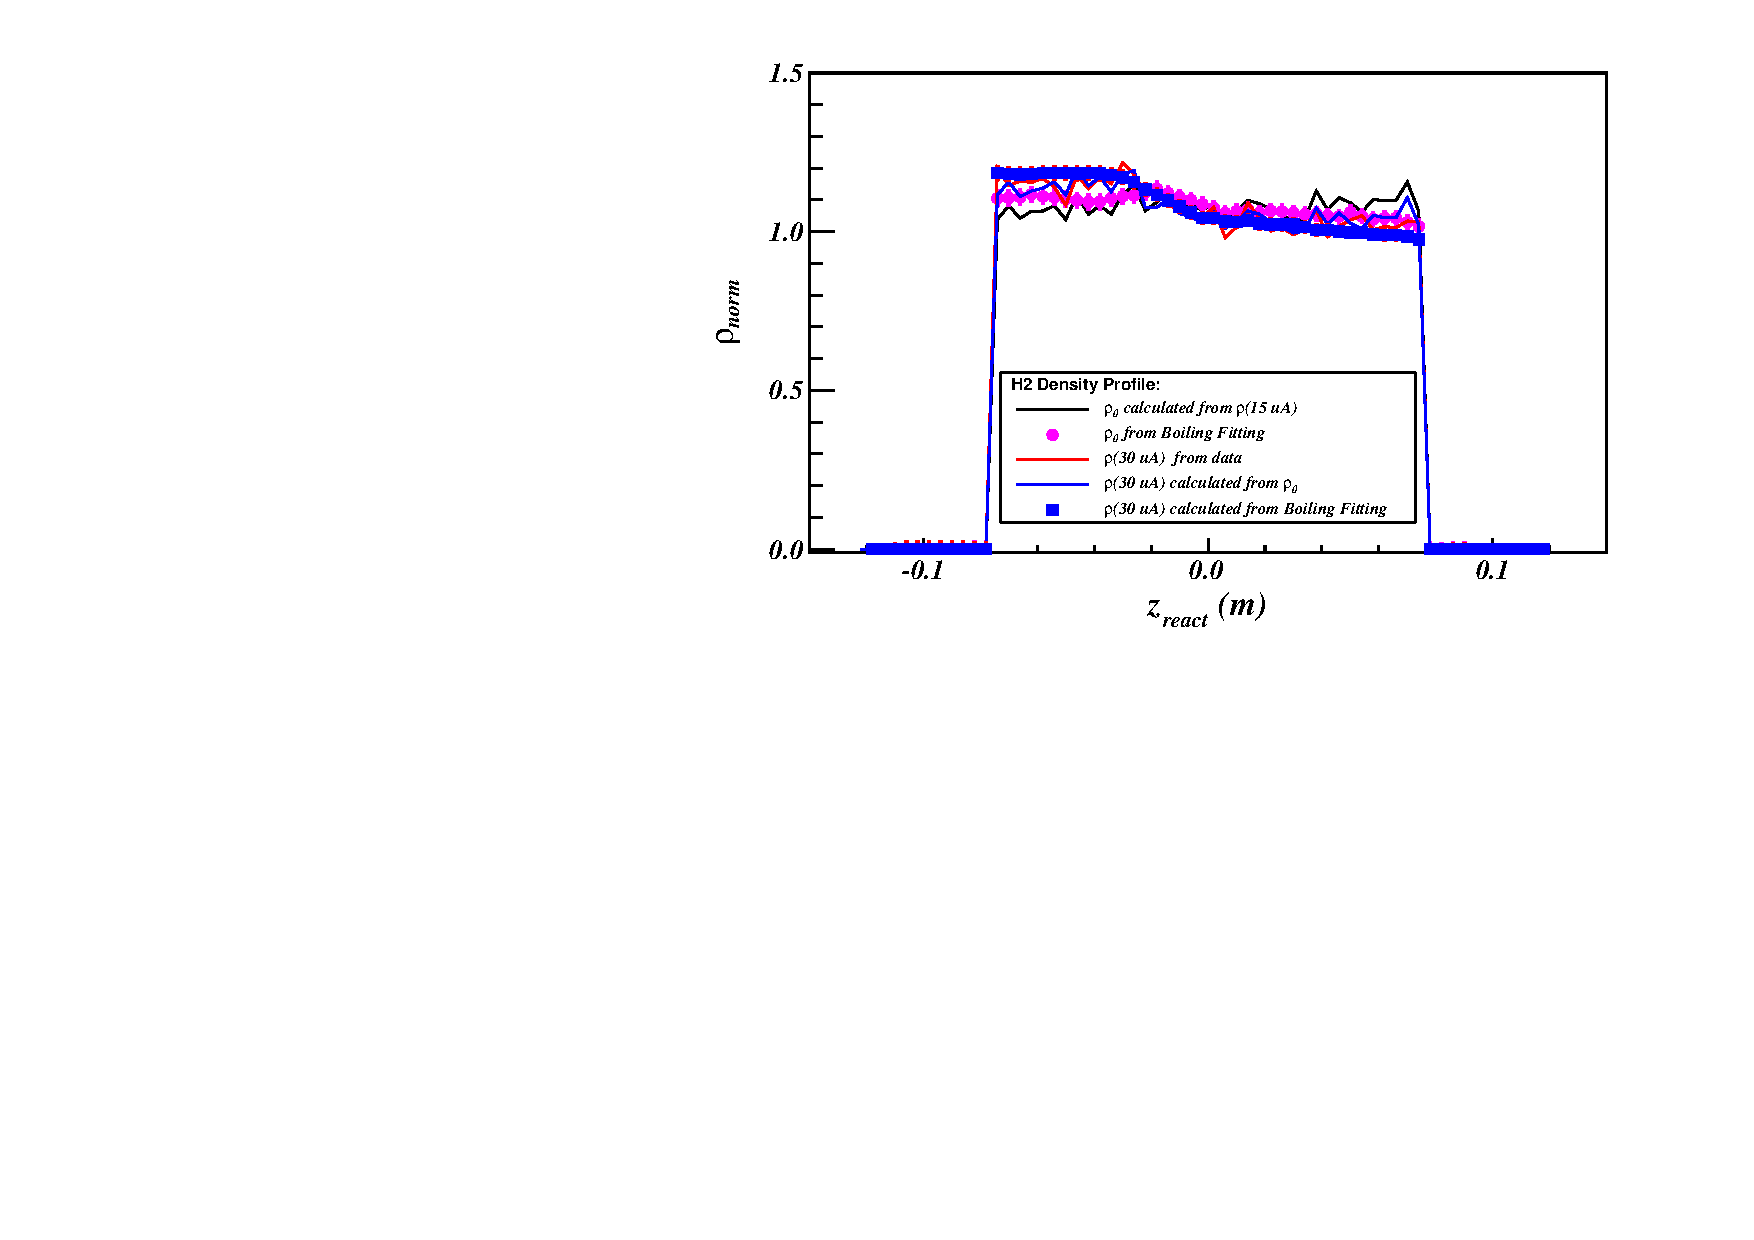
\includegraphics[type=pdf,ext=.pdf,read=.pdf,width=0.45\textwidth]{./figures/cryo/H2_Check_30} 
    }
    \hfill
    \subfloat[$\mathrm{^{2}H}$ at I=45 uA]{
      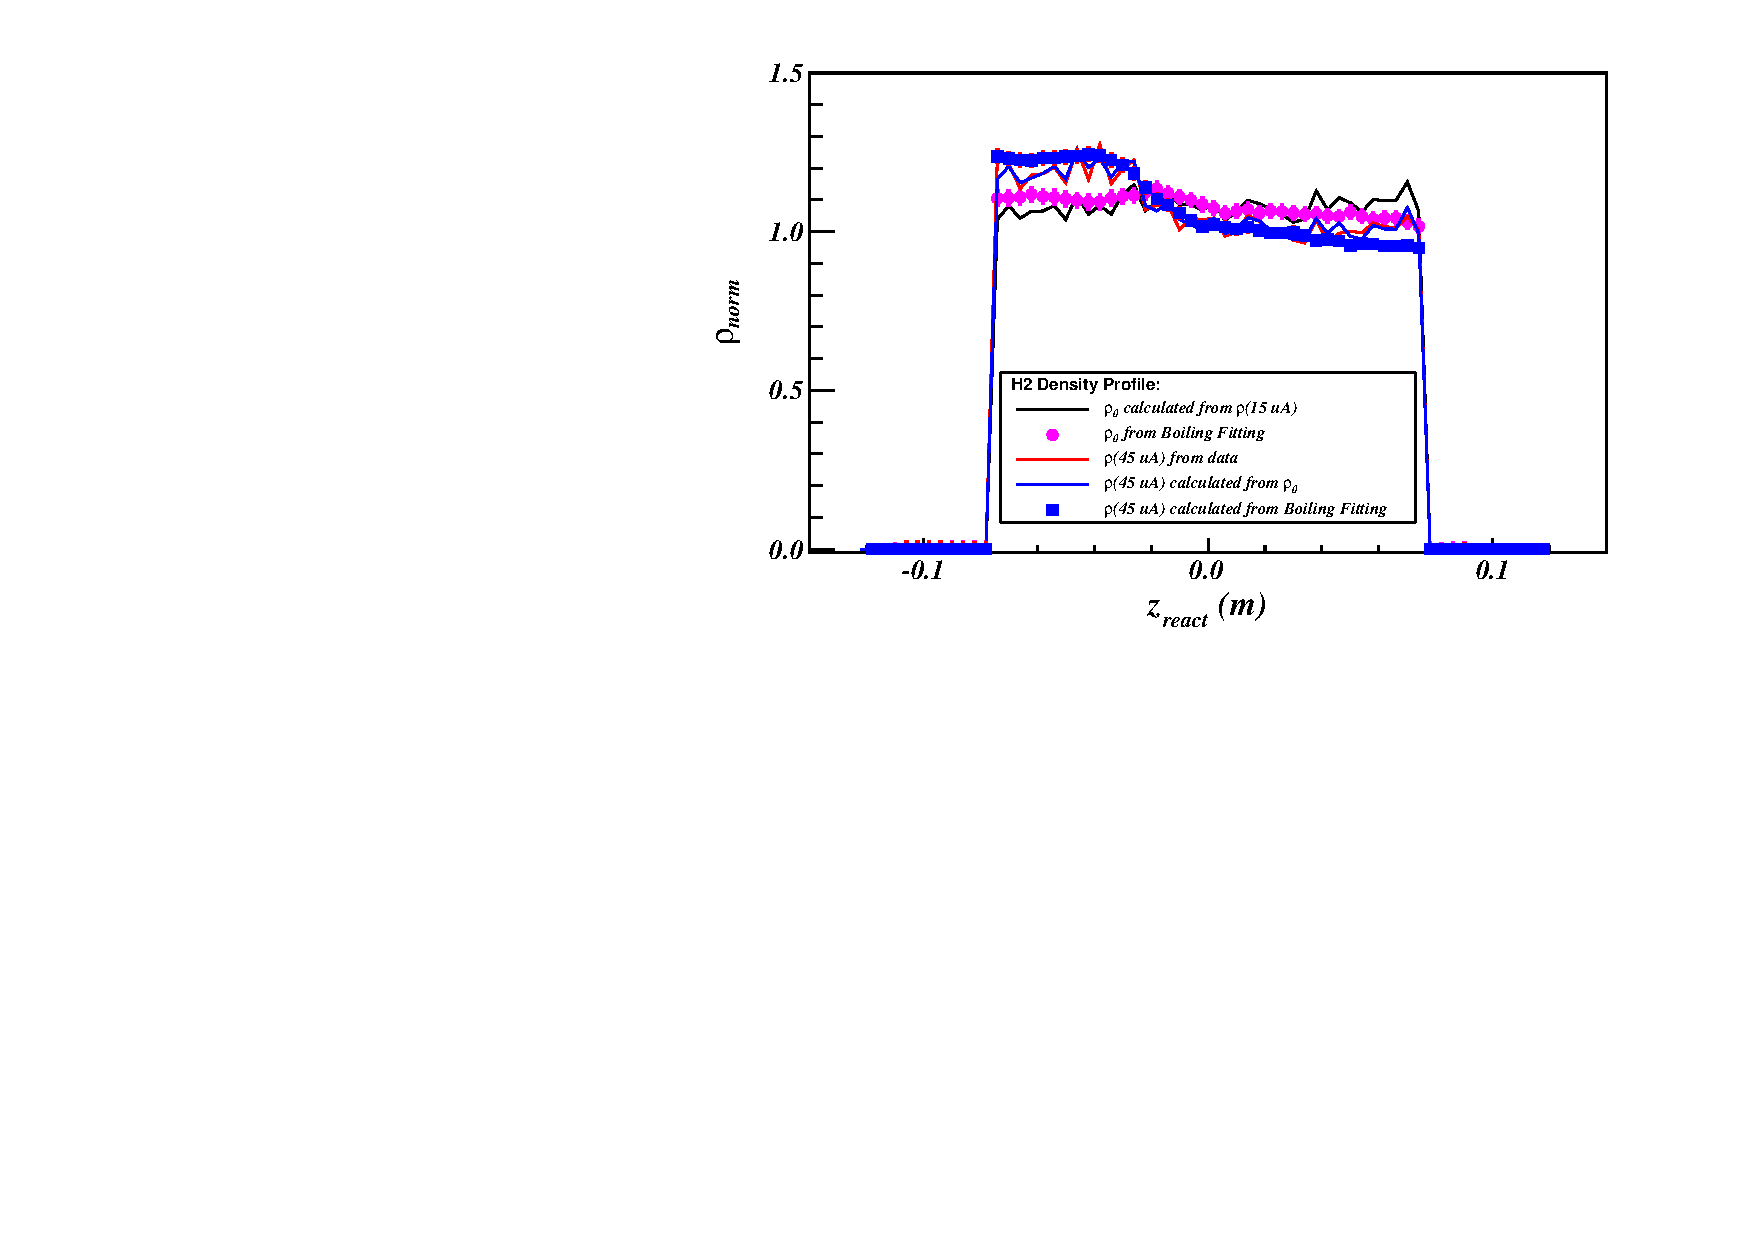
\includegraphics[type=pdf,ext=.pdf,read=.pdf,width=0.45\textwidth]{./figures/cryo/H2_Check_45} 
    }
\\
    \subfloat[$\mathrm{^{3}He}$ at I=60 uA]{
      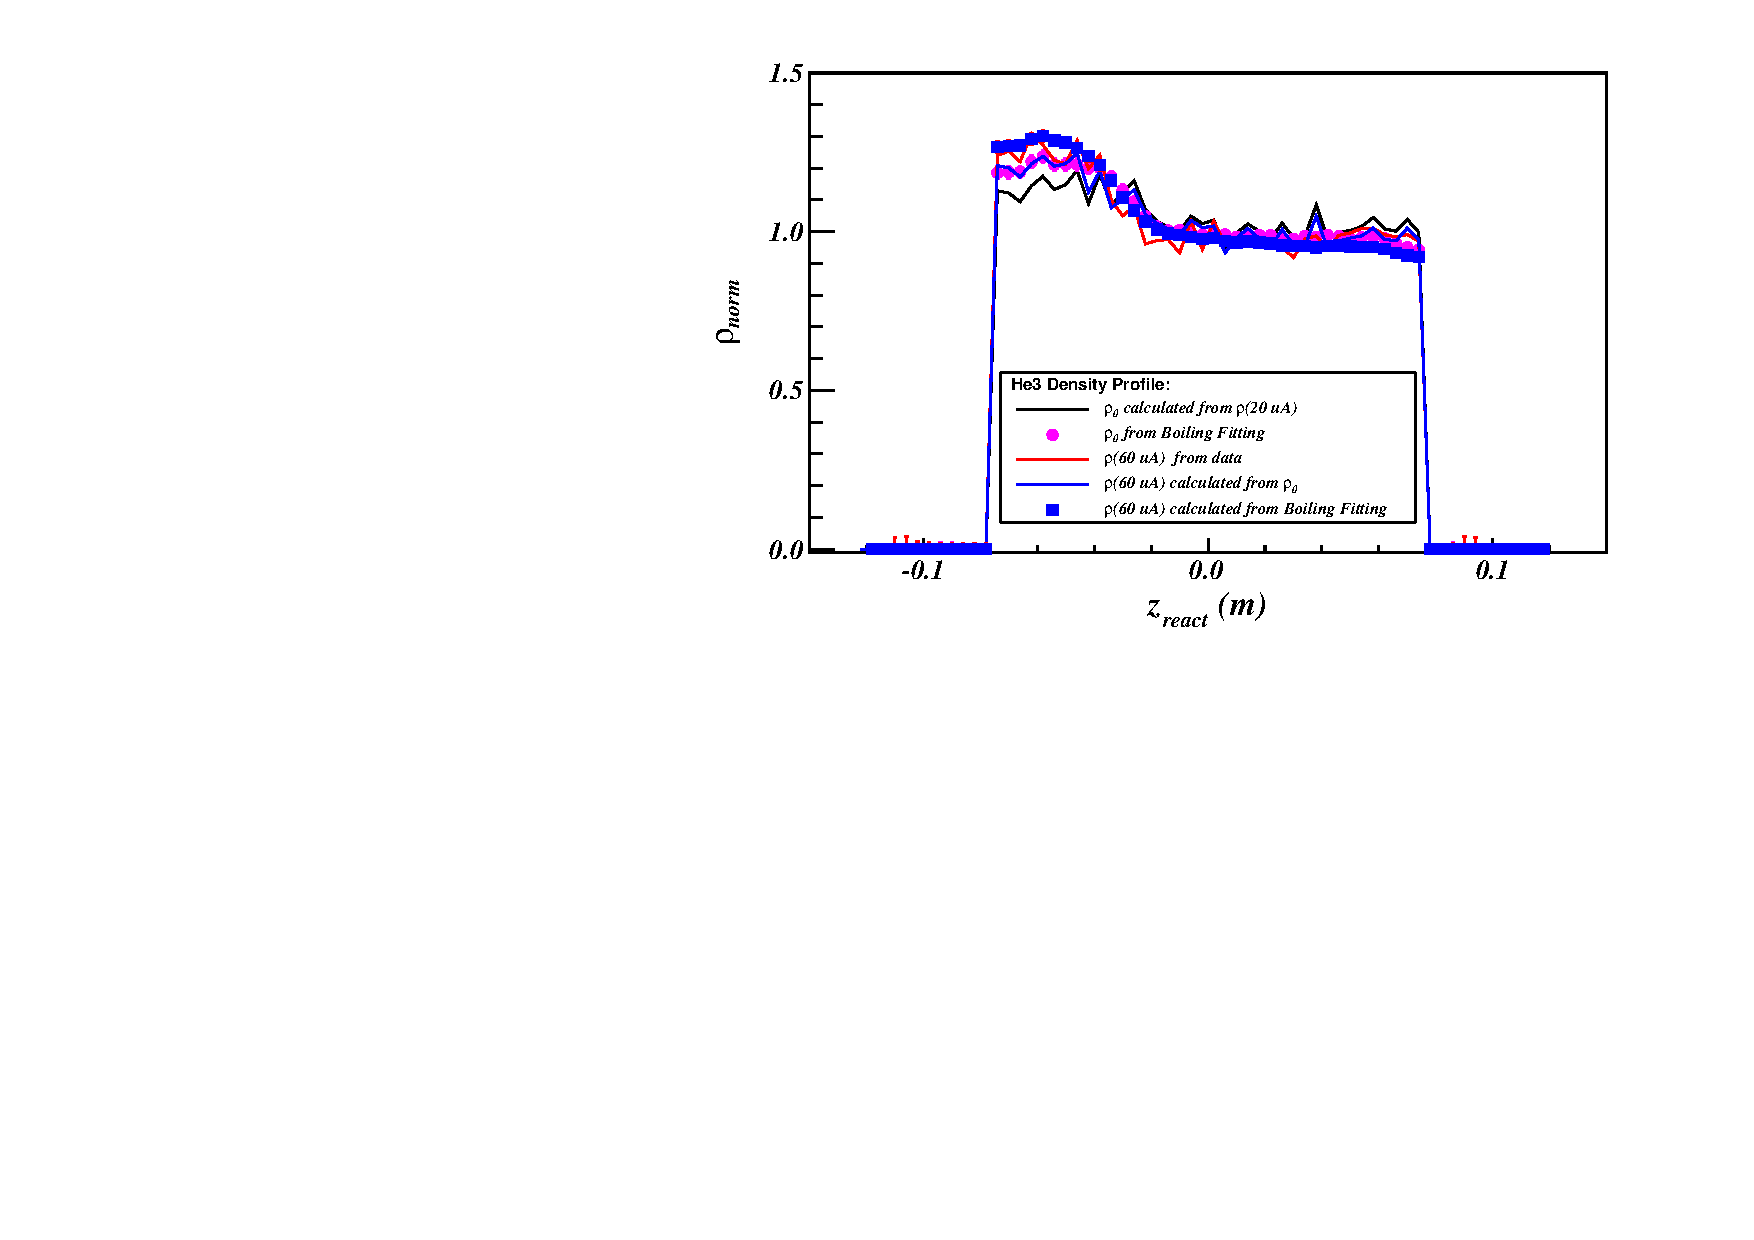
\includegraphics[type=pdf,ext=.pdf,read=.pdf,width=0.45\textwidth]{./figures/cryo/He3_Check_60} 
    }
    \hfill
    \subfloat[$\mathrm{^{3}He}$ at I=120 uA]{
      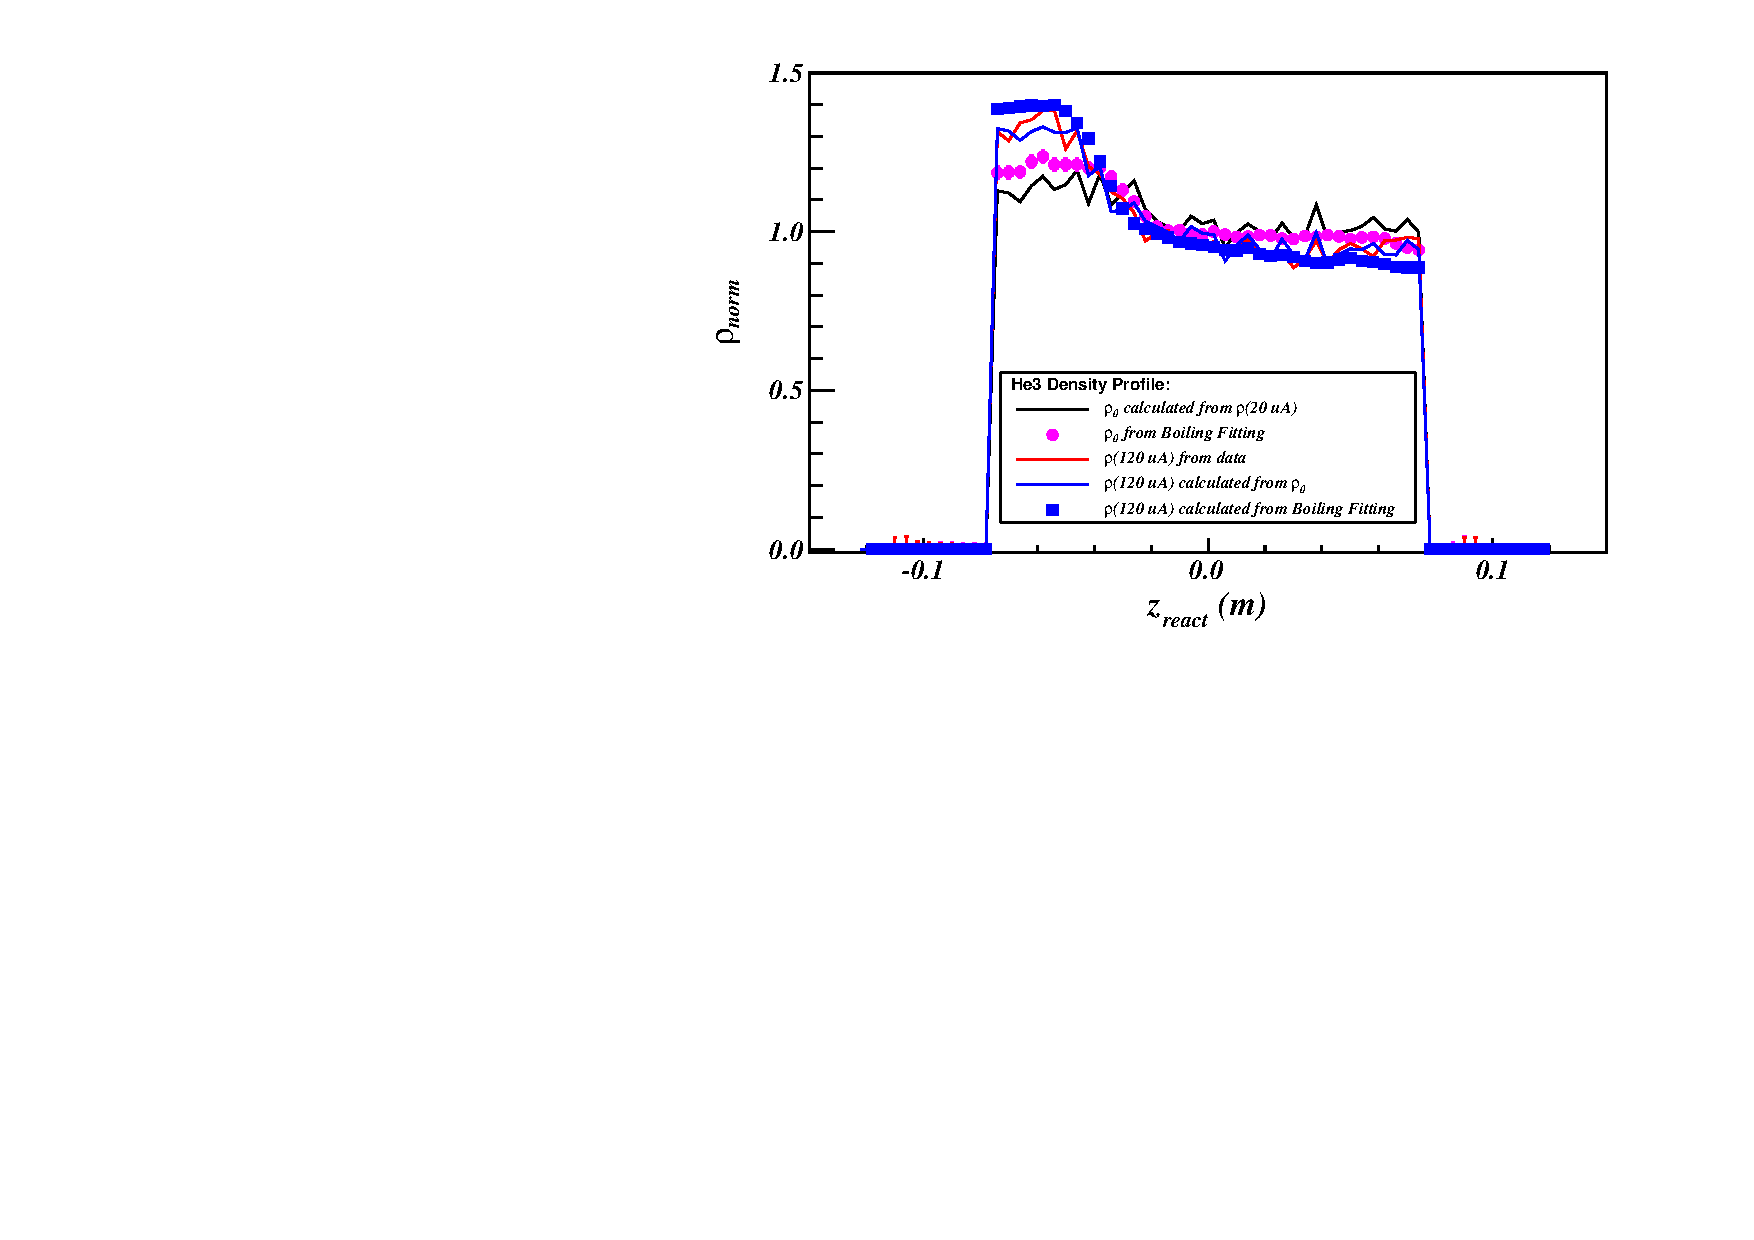
\includegraphics[type=pdf,ext=.pdf,read=.pdf,width=0.45\textwidth]{./figures/cryo/He3_Check_120} 
    }
\\
    \subfloat[$\mathrm{^{4}He}$ at I=60 uA]{
      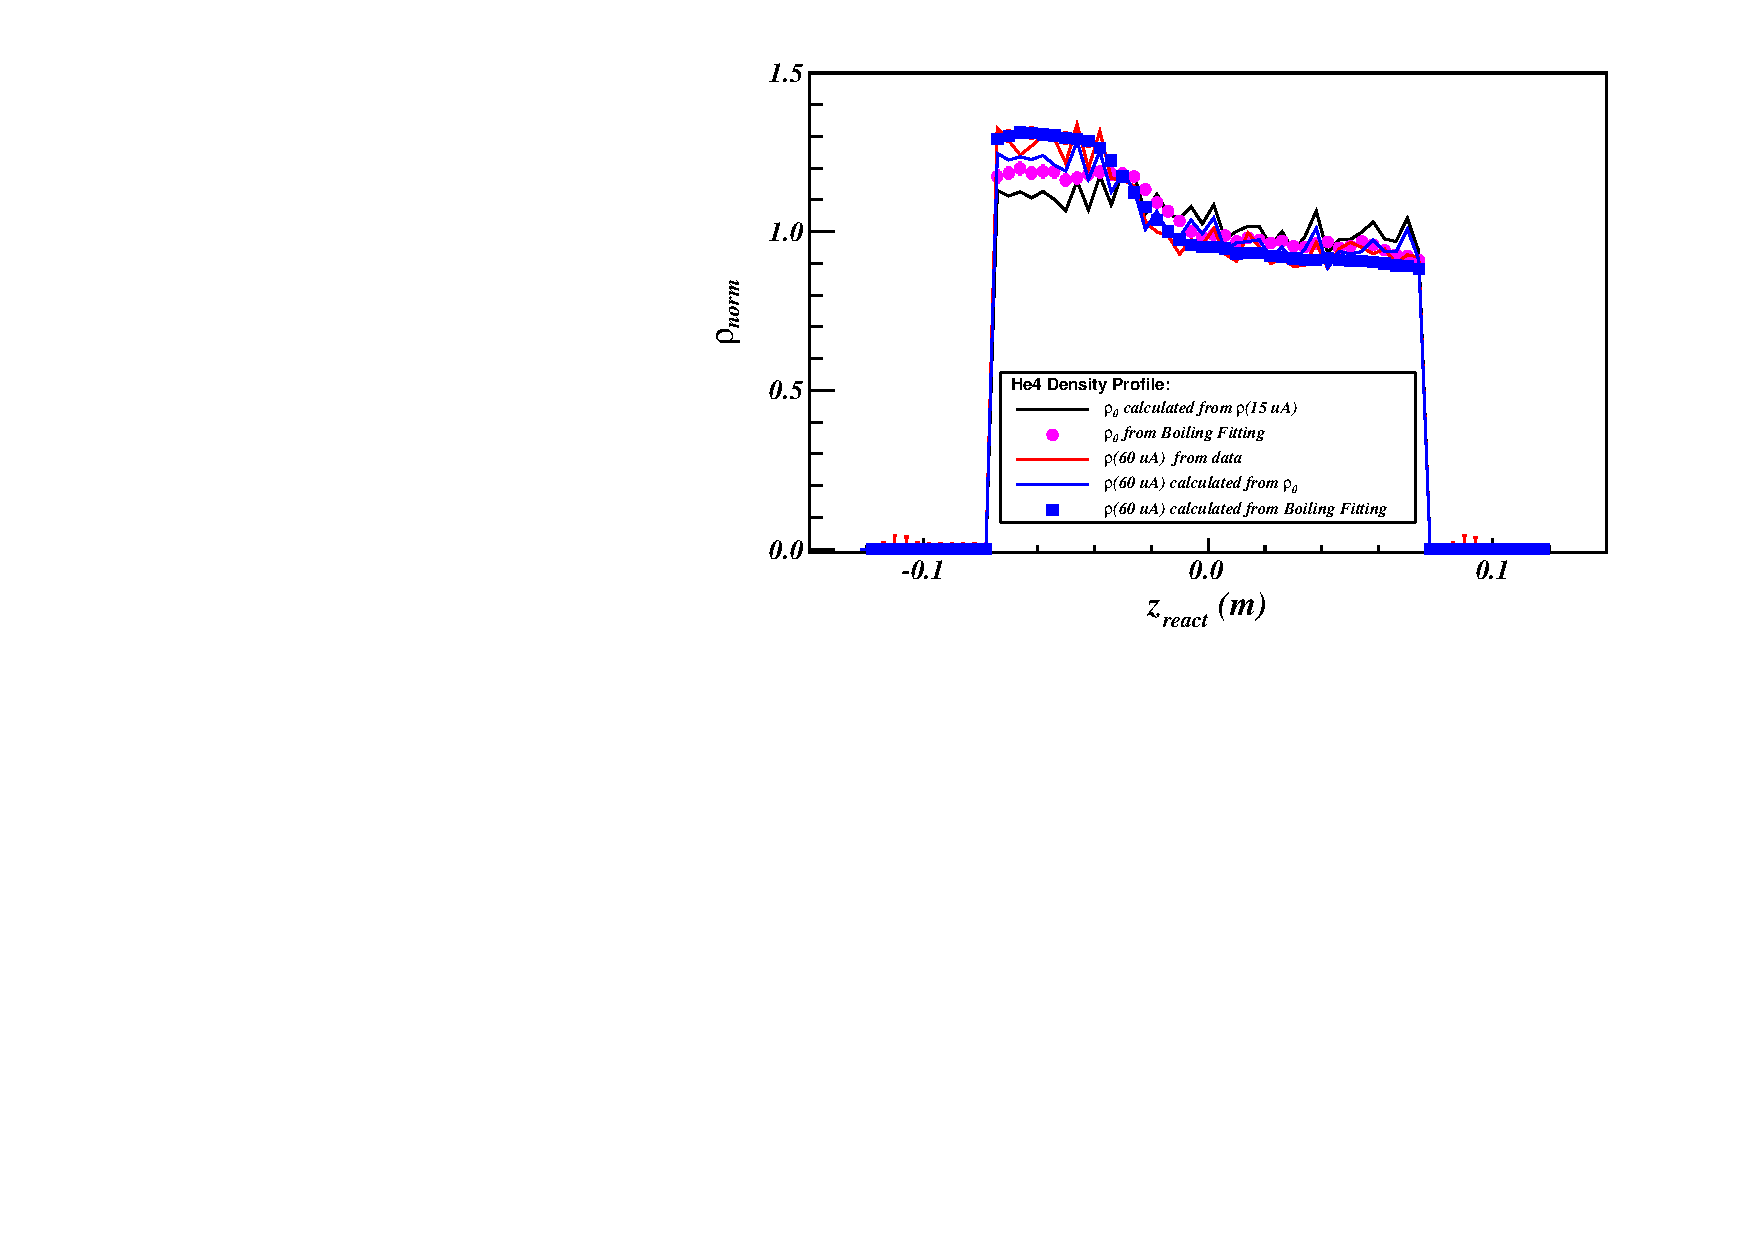
\includegraphics[type=pdf,ext=.pdf,read=.pdf,width=0.45\textwidth]{./figures/cryo/He4_Check_60} 
    }
    \hfill
    \subfloat[$\mathrm{^{4}He}$ at I=95 uA]{
      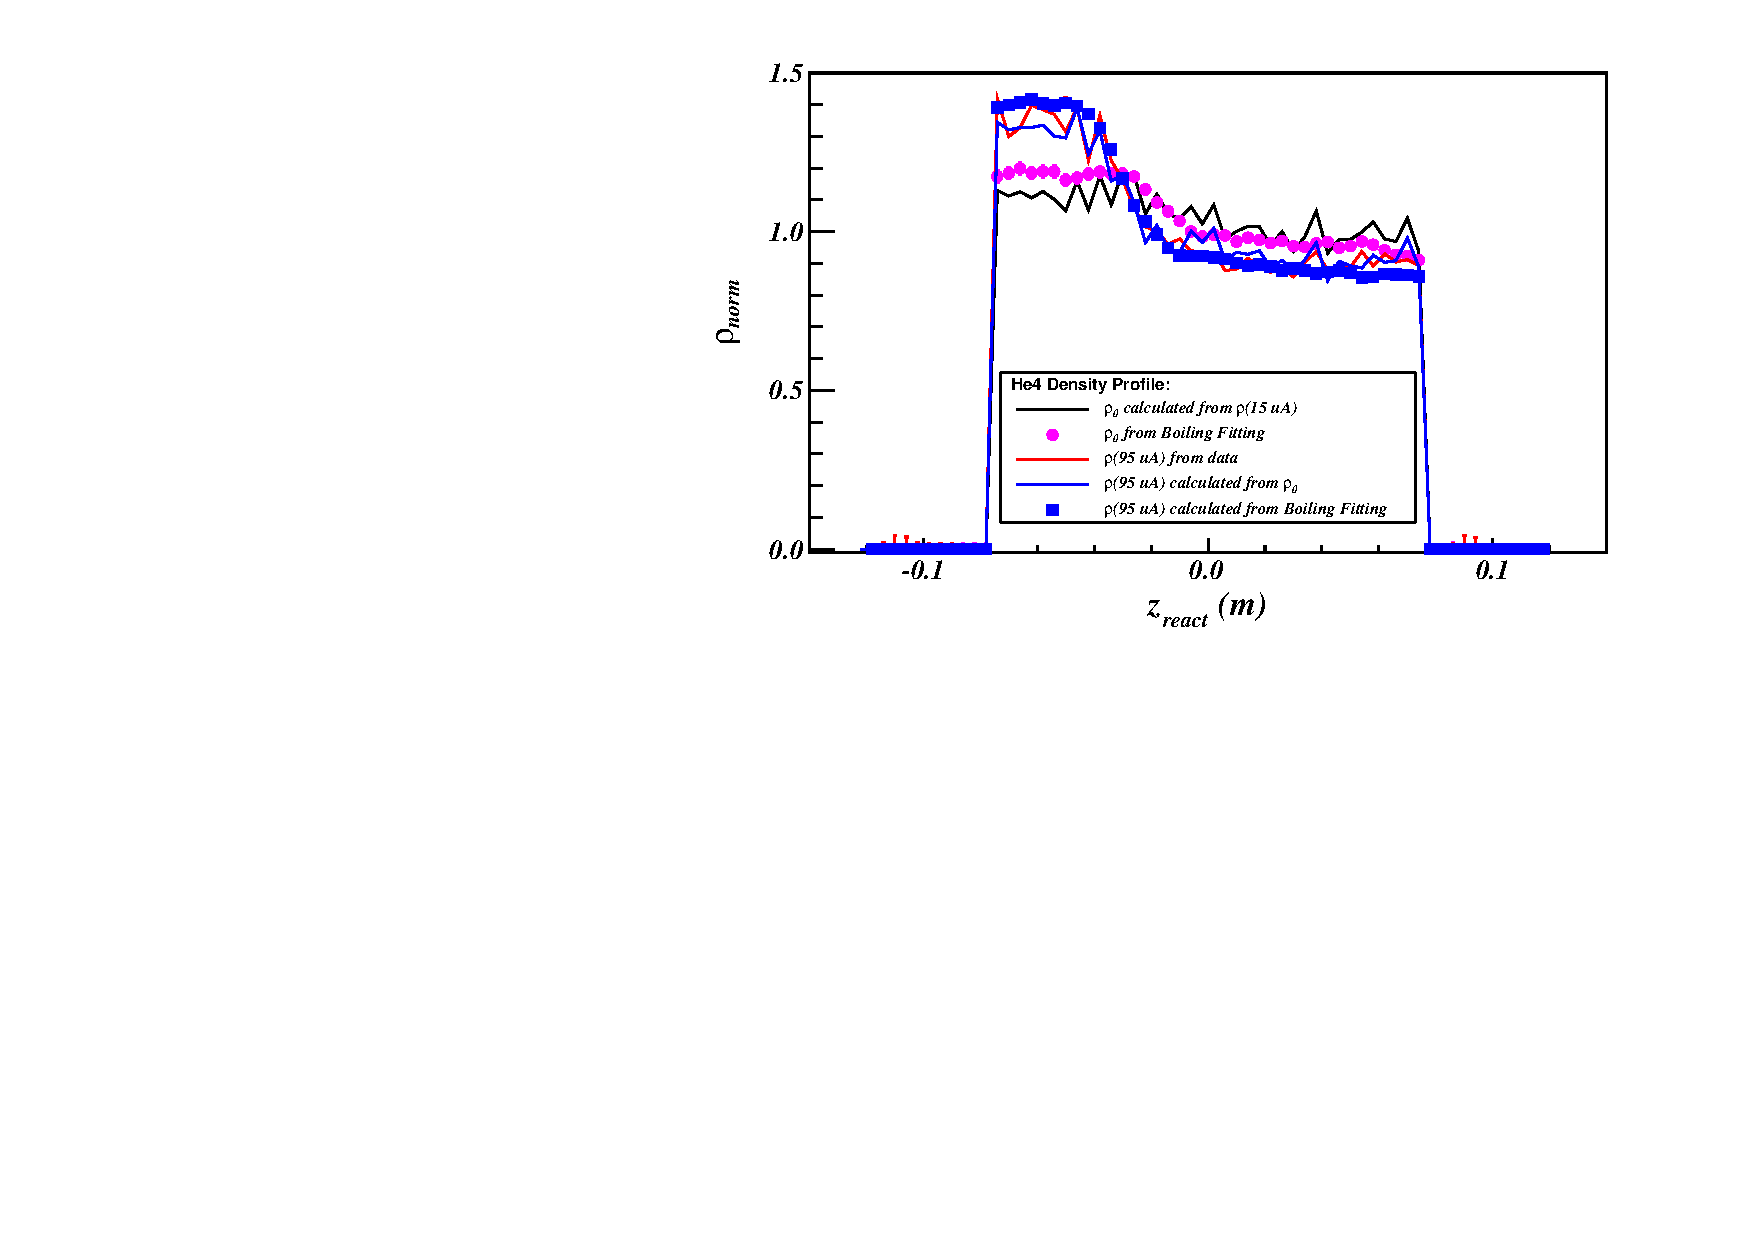
\includegraphics[type=pdf,ext=.pdf,read=.pdf,width=0.45\textwidth]{./figures/cryo/He4_Check_95} 
    }
    \caption[Cryo-targets relative density distribution]{\footnotesize{Cryo-targets relative density distribution extracted from data and corrected by the boiling factors. The density values were calculated in each $z_{react}$ bin and the peaks in these distribution were due to the statistical fluctuation. To remove the contribution of the endcaps, a cut was apply on the target length, $\mathrm{|z_{react}|\leq 7.5~cm}$}}
    \label{cryo_den_comp}
  \end{center}
\end{figure}

 Fig.~\ref{cryo_den_comp} also compares the distributions of the target density obtained from the boiling study and from the method discussed in this section. Ignoring the statistical fluctuations of the histograms, both methods give similar density profiles, and the small difference can be explained by the errors of the HRS acceptance simulation in SAMC and the cross section model in XEMC.
 
\section{Absolute Density}
 When the density distribution is uniform, the absolute density of a cryo-target can be calculated with the temperature and pressure readings from the target system with the fixed volume of the target cell. However, the calculation becomes impossible when the density is not uniform since the temperature and pressure fluctuate inside the target. While the relative density distribution has been extracted as discussed in previous section, one can obtain the absolute density distribution by calculating the density at the entrance of the target cell where the temperature and pressure were monitored.
 
  Whereas, the extracted relative density distribution at the entrance does not reflect the true density profile of the cryo-target due to the contamination of the aluminium endcaps during the boiling study, and an assumption has been made to assign the density value at the entrance to the value at $\mathrm{-10\leq z_{react} \leq -7.5~cm}$. The true value should not deviate too far away from this value since this location is very close to the entrance and the coolant flow should be able to maintain the same temperature as it at the entrance. The deviation can be corrected when comparing the experimental yield and the simulation yield, while the last one, yet, depends on the cross section model. To obtain the accurate density, one can utilize the 2N-SRC plateaus of cross section ratio of the carbon target to the cryo-targets~\cite{SLAC_Measurement_PRC.48.2451,PhysRevLett.96.082501,PhysRevLett.108.092502}, which have been well measured in previous experiments. Table~\ref{cryo_density_table} gives the densities of cryo-targets at the entrance and the yield-normalized density at $\mathrm{z_{react}=7.5~cm}$, where the values will be updated when they are further normalized by the 2N-SRC plateaus.
\begin{table}[htbp]
 \begin{tabular}{lcccccccc}
 \toprule
 Target:                        & $\mathrm{^{2}H}$  & $\mathrm{^{3}He}$-I  & $\mathrm{^{3}He}$-II & $\mathrm{^{4}He}$ \\
 \midrule
 $\rho_{entrance}~(g/cm^{3})$:   & 0.1676   & 0.0213      &  0.0296     & 0.0324 \\
 $\rho_{z_{react}=-7.5~cm}~(g/cm^{3})$:&  0.1906  & 0.0210 &  0.0292    & 0.0280 \\
 \bottomrule
 \end{tabular}
% \centering
\caption[Cryo-targets densities]{\footnotesize{Cryo-targets densities, where two values of the $\mathrm{^{3}He}$ density refer to two different run periods. The values of $\rho_{entrance}$ are calculated from the temperature and pressure reading~\cite{target_report}. The values of $\rho_{z_{react}}=-7.5~cm$ are the values of $\rho_{entrance}$ normalized by the ratio of the experimental yield and the simulation yield and will be further corrected by comparing the 2N-SRC plateaus.}}
\label{cryo_density_table}
\end{table}

\section{Radiative Correction}
  The most essential parameter during the radiative correction is the radiation length of the target. For a uniform target, the radiation length is evaluated at the center of the target. For a non-uniform target, such an approximation has to be carefully examined. 

\begin{figure}[!ht]
 \begin{center}
  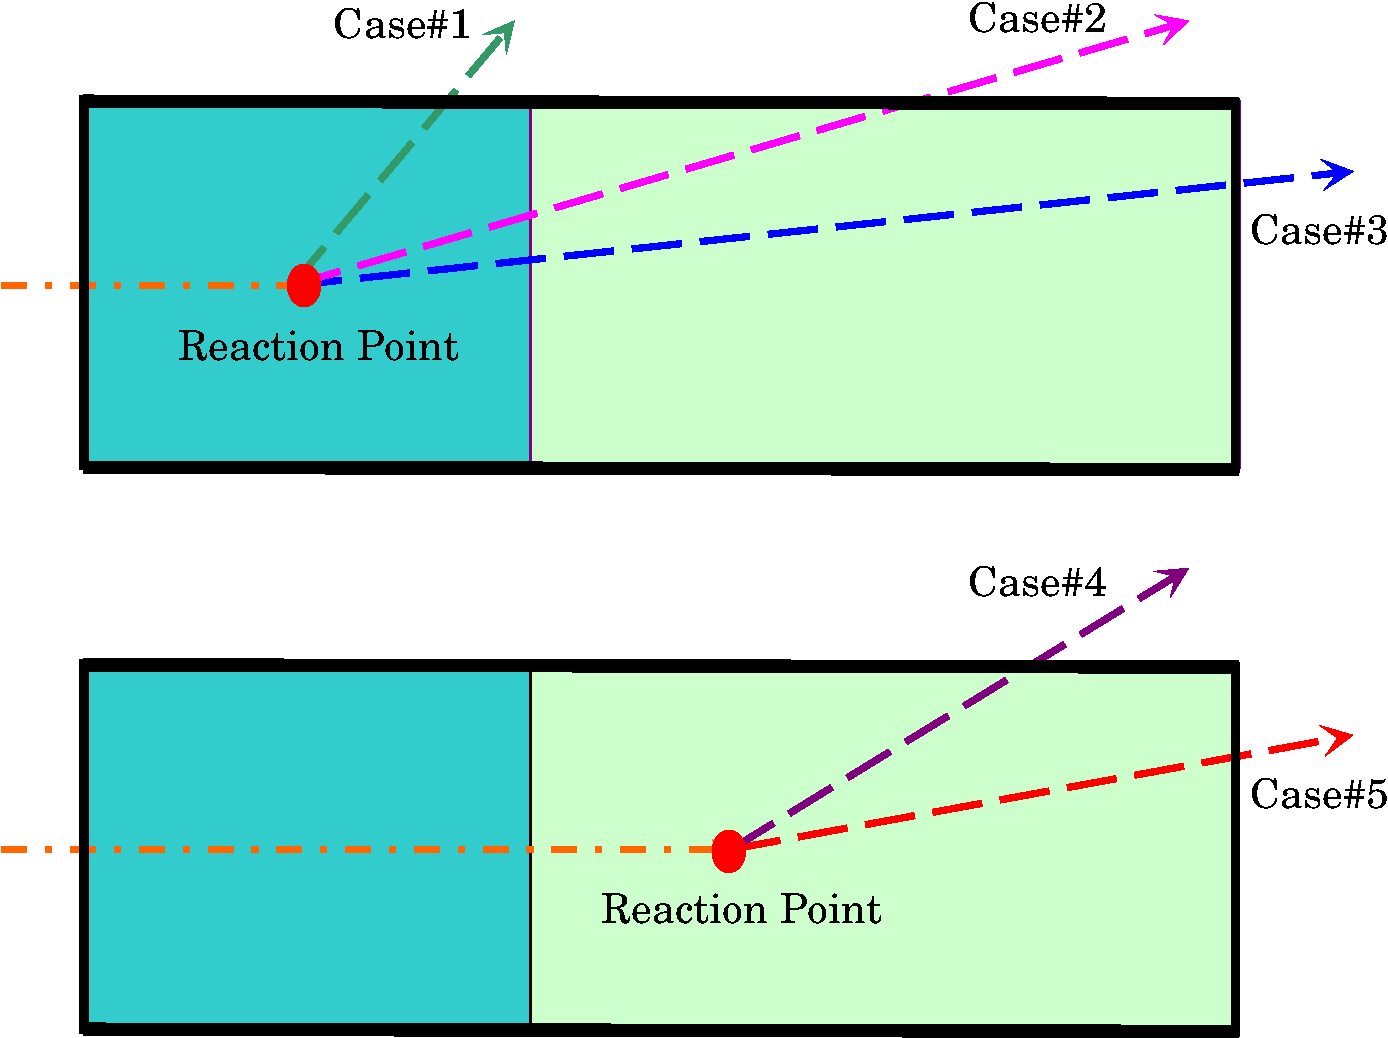
\includegraphics[angle=0,width=0.6\textwidth]{./figures/xemc/radc_cases}
  \caption[Different cases to calculate the radiation lengths]{\footnotesize{Different cases to calculate the radiation lengths, where the target has two parts with different density. The target cell's entrance, exit and wall (black lines ) also have different thickness. Depending on the reaction point in the forward scattering, there are five cases which give different radiation lengths.}}
  \label{radc_cases}
 \end{center}
\end{figure}
  In the radiative correction model in XEMC, the density distribution of a cryo-target is simplified as a step function, where the density is 30\% higher for -10~cm$\mathrm{\leq Z_{react}}\leq$-2~cm and is 20\% lower for the rest of the target. The value of radiation length in such a distribution depends on the reaction location and the scattering angle. Fig.~\ref{radc_cases} gives 5 different scattering paths which have been coded in the model. 
  
 \begin{figure}[!ht]
\begin{center}
  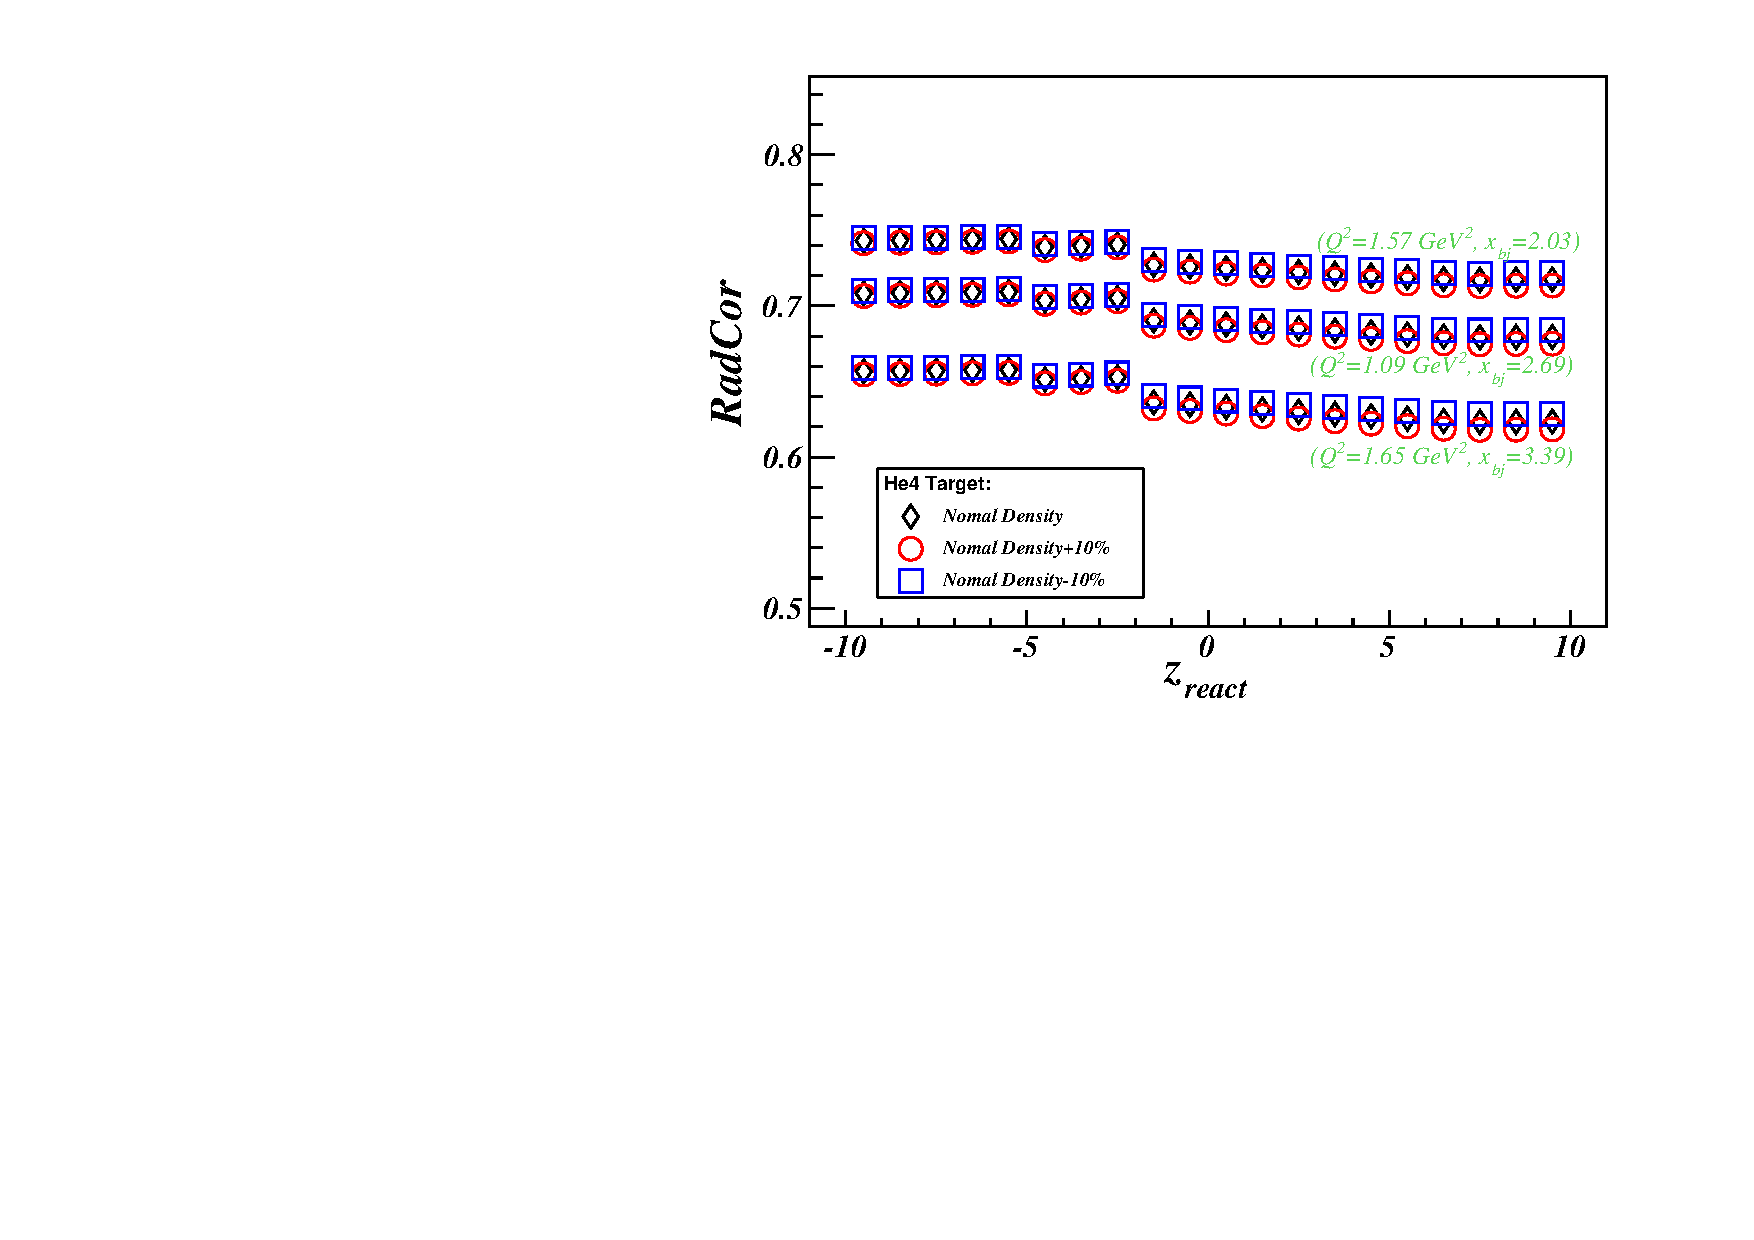
\includegraphics[angle=0,width=0.8\textwidth]{./figures/xemc/He4_RadC}
  \caption[Position dependence of radiative effect on $\mathrm{^{4}He}$]{\footnotesize{Position dependence of radiative effect on $\mathrm{^{4}He}$. With a step function as the density distribution, $\mathrm{z_{react}}$ was divided into 20 bins where in each bin radiative correction factors were calculated at three different kinematic settings. To check the variation of the absolute density, the radiative effect was calculated in each $\mathrm{z_{react}}$ bin by changing the density by $\mathrm{\pm 10}$\%. The radiative effect clearly depends on the reaction location but has small dependence on the absolute density.}}
  \label{he4_rad_check}
 \end{center}
\end{figure}
  To study the position dependence of the radiative effect, the target was divided into 20 bins along the $\mathrm{z_{react}}$ distribution where the radiative correction factor (Eq.~\eqref{eq_radc_fact}) was calculated in each bin. Fig.~\ref{he4_rad_check} shows the distribution of the radiative correction factor as a function of $\mathrm{z_{react}}$. The downstream part of the target has stronger radiative effect since the incoming electron loses more energy while passing through the upstream part which has higher density. Overall, the variation of the radiative correction factors along the target length is less than 2\%. The distributions at different kinematic settings were also studied by changing the value of $E'$ by $\mathrm{\pm}$ 3\%. The results give the similar distribution which indicates that the $\mathrm{z_{react}}$-dependence of the radiative correction factors does not change much within one kinematics.
  
   The absolute target density varies with the beam current. Even though the beam current was set to a constant value for each target, it still had fluctuations depending on the stability of the beam. As discussed in the previous section, the absolute density for cryo-targets will be further normalized by the 2N-SRC ratio. In Fig.~\ref{he4_rad_check}, the radiative effect at different target densities was also examined and the results showed very small deviation when changing the density by  $\mathrm{\pm}$ 10\%.
   
% As discussed in Section 5.7, the radiated cross section was not calculated event-by-event during the cross section extract. Instead, a cross section table was generated by dividing the entire kinematic space into grids, and one looked for the cross section value from the table for each event. This method can dramatically increase the speed of calculation but one has to evaluate the radiative correct at the center of the target with the uniform density equal to the average value of the whole target. For uniform targets this method is approximately accurate. However, when the target density is non-uniform, more events come from the dense part of the target which has stronger radiative effect. 
    
% The radiative correction factor at a position on $\mathrm{z_{react}}$ was weighted by the relative density in this location, and the average value of all these factors was compared with the value calculated at the center of the target after assuming the target to be uniform and its density equal to the average density. The study showed a X\% difference between this two values.